% !Mode:: "TeX:UTF-8"
%!TEX program  = xelatex
% 编译：xelatex -> bibtex -> xelatex -> xelatex
\documentclass[bwprint]{gmcmthesis}

\usepackage{tikz}
\usetikzlibrary{arrows.meta,positioning,calc,fit,backgrounds}
\usepackage{algorithm}
\usepackage{algpseudocode}
\usepackage{csvsimple}
\usepackage{float}
\normalem % ulem 默认会把 \emph 变成下划线，这里恢复成正常强调
\AtBeginEnvironment{table}{\small\setlength{\tabcolsep}{4pt}} % 表格用五号左右字号
\setcounter{tocdepth}{2}
\setlength{\emergencystretch}{2em}

% 待填项：用醒目的红字标出，提交前务必全部替换
\newcommand\todo[1]{\textcolor{red}{\textbf{【待填：#1】}}}

\renewcommand{\algorithmicrequire}{\textbf{输入：}}
\renewcommand{\algorithmicensure}{\textbf{输出：}}
\floatname{algorithm}{算法}

\title{多模态情感特征对齐与鲁棒可解释预测}
\baominghao{26XXXXXXXXX} % 参赛队号
\schoolname{XX大学}      % 学校名称
\membera{XXX}            % 队员A
\memberb{XXX}            % 队员B
\memberc{XXX}            % 队员C

% ------------------------------------------------------------------
% 封面与摘要页标题：模板原图写的是“第十五届”，这里改成文字版第二十三届；
% logo.pdf 下排是 2018 年承办单位和第十五届标识，裁掉只留上排三个。
% 如拿到当届官方封面，直接替换即可。
% ------------------------------------------------------------------
\makeatletter
% 模板的 \thesection 自带尾点，交叉引用会变成“第5.章”，这里把点挪到标题格式里
\renewcommand\thesection{\arabic{section}}
\newcommand\secdot{.}
\def\@seccntformat#1{\csname the#1\endcsname\csname secdot@#1\endcsname\ \ }
\def\secdot@section{\secdot}
\newcommand\tocsecdot{.}
\titlecontents{section}[0pt]{\vspace{2mm}\bfseries\heiti}
  {\thecontentslabel\tocsecdot\hskip.5em}{}{\titlerule*[0.5pc]{.}\contentspage}
\renewcommand\gmcm@ges@string@contents{%
  {\zihao{-2}中国研究生创新实践系列大赛}\\[6pt]
  “华为杯”第二十三届中国研究生\\[2pt]
  数学建模竞赛}
\def\ge@maketitle{%
  \newpage
  \if@gmcm@preface
  \setcounter{page}{0}%
  \def\thepage{0}%
  \thispagestyle{empty}%
  \begin{center}
    {
\includegraphics[trim=0 95 0 0,clip]{logo}}
    \vskip2.2cm
    {\xinwei\zihao{2} \gmcm@ges@string@contents \par}
  \end{center}
  \vskip2em
  \renewcommand\arraystretch{1.3}%
  \noindent\begin{tabularx}{\textwidth}{lX}
    \zihao{-2}\bfseries 学\qquad 校&\zihao{-2}\bfseries\gmcm@tokens@schoolname\\
    \hline\\[-15pt]
    \zihao{-2}\bfseries 参赛队号&\zihao{-2}\bfseries\gmcm@tokens@baominghao\\
    \hline\\[-15pt]
    \multirow{3}{*}{\zihao{-2}\bfseries 队员姓名}&\zihao{-2}\bfseries 1. \gmcm@tokens@membera\hfill\null\\
    \cline{2-2}\\[-15pt]
    &\zihao{-2}\bfseries 2. \gmcm@tokens@memberb\hfill\null\\
    \cline{2-2}\\[-15pt]
    &\zihao{-2}\bfseries 3. \gmcm@tokens@memberc\hfill\null\\
    \hline
  \end{tabularx}
  \fi
  \makenametitle}
\def\makenametitle{%
  \newpage
  \setcounter{page}{1}%
  \vspace*{-1.2cm}
  \begin{center}
    {\xinwei\zihao{3} \gmcm@ges@string@contents \par}
  \end{center}
  \vskip0.2cm
  \begin{center}\begin{tabularx}{.95\textwidth}{@{}lX@{}}
    {\zihao{4} 题\qquad 目} &\hfill\zihao{3}\heiti \@title\hfill\null\\
    \cline{2-2}
  \end{tabularx}\end{center}
  \vskip-0.4cm}
\makeatother

\begin{document}

\maketitle

\begin{abstract}
真实场景中，文本、语音、视觉三路信号时间尺度不一，还常常局部缺失，而多数情感模型只给结论、不给依据。本文围绕特征对齐、缺失下的鲁棒预测和可解释预测三项任务，建立了从原始视频到可核验结论的完整流程。

针对问题一，本文用 bert-base-uncased、librosa 和 YuNet 从附件1的100条视频中提取768、74、35维的文本、语音、视觉特征，再用三角核重采样对齐到统一的50个位置，给出按词位置（口径H，与附件2一致）、全程50等分、说话者有效时段50等分三种方案。第三种是本文的改进：以“说话者的脸是否可见”划定有效时段，既剔除无人时段，又保留不说话时的表情。100条样本平均保留93\%的时长，语音、视觉非零位置分别为48.0和47.5，而按声音判定只有32\%的时长在说话。

针对问题二，核查发现附件2的零帧绝大多数是尾部填充（语音96.28\%、视觉89.18\%），没有句中连续缺失，与附件3的形态不符。以语言主导融合与自蒸馏模型（LDSD）为基线（完整模态 Acc-3 68.78\%、F1 60.48\%），从5个候选模块中筛出连续段缺失增强与超模态补洞，得到 LDSD-Seg：段缺失 F1 由47.26\%升至61.70\%，MAE 由0.7112降至0.6639，验证集上完整与段缺失的 F1 落差由15.6个点缩小到0.1个点。108个单元的三因子扫描表明缺失时长是主因：语言缺失90\%以内 MAE 仅增0.060，全缺时增0.789；语音、视觉的影响低于0.006，位置的影响不到0.003。附件3预测为正向14条、负向11条、中性5条。

针对问题三，利用附件2中序列位置与 BERT 词元一一对应的关系，在不改网络的前提下构建帧—词元回指、干预式模态归因、滑动窗口片段扫描和证据呈现四层解释。忠实性比值为2.88，加噪稳定性 Spearman 系数为0.9973；验证集中92\%的样本以文本为主导，与模态消融结果一致。附件4的20条样本主导模态均为文本，可找回真值的5条极性全对、强度 MAE 为0.3334，但预测强度普遍偏大。

\keywords{多模态情感分析\quad 时序对齐\quad 说话者人脸跟踪\quad 模态局部缺失\quad 自蒸馏\quad 干预式归因}
\end{abstract}

\pagestyle{plain}
\tableofcontents
\newpage

% ==================================================================
\section{问题重述}
% ==================================================================

\subsection{问题背景}

人在表达情绪时很少只靠一种信号：说了什么（文本）、怎么说的（语调、停顿）、说话时的表情，三者共同决定了一句话的情感色彩。多模态情感分析就是把这几路信号放在一起建模，它是具身智能、人机对话等应用绕不开的环节。

落到实际数据上，首先要解决的是“对齐”：文本以词为单位、没有时间戳，语音按毫秒分帧，视频按固定帧率抽帧，三路信号的时间尺度各不相同，必须先统一到同一套序列位置上，下游模型才能使用。在此基础上，还有两个问题特别常见。第一个是缺失：镜头被挡住几秒、背景噪声盖过了人声、语音转写漏掉了半句，都会让某一路信号在一段时间里“空掉”。很多融合模型默认三路输入都在，一旦某路局部为空，性能会掉得很厉害。第二个是可信度：模型给出“负向、强度$-1.1$”之后，使用者往往想知道它凭的是哪句话、哪一段声音或哪几帧表情，而大多数模型给不出可核对的依据。

赛题以 CMU-MOSEI 英文多模态情感数据集\cite{zadeh2018mosei}为基础，要求依次完成特征提取与时序对齐、模态局部缺失下的鲁棒预测、可解释预测三项任务，本文依次完成这三项任务。已有的经典融合方法，如张量融合网络 TFN\cite{zadeh2017tfn}、低秩融合 LMF\cite{liu2018lmf} 和跨模态 Transformer MulT\cite{tsai2019mult}，都以组织好时序的三模态特征为输入\cite{zhang2024review}，因此问题一所做的特征提取与对齐是后两问的前置环节。

\subsection{数据说明}

赛题共提供四个附件。附件1是从 CMU-MOSEI 中选出的100条原始英文视频，按原始视频编号 video\_id 分为37个子文件夹，每个片段以 clip\_id.mp4 保存，时长2.648～34.567秒；配套的标注表给出每条片段的转写文本、连续情感强度和极性标签，用于问题一。附件2是整理好的 CMU-MOSEI 特征文件，含对齐版（aligned\_50.pkl）与非对齐版两套，每套4850条样本，按训练、验证、测试划分，带有情感极性（负向、中性、正向）和连续强度（$[-3,3]$）两种标签。附件3是30条无标签的“模态局部缺失专项测试集”，缺失表现为某些模态中特征值全为零的连续区间。附件4是20条无标签的“可解释性专项测试集”，三模态完整，另附原始视频。赛题规定问题二、问题三的模型只能在附件2的训练集上学习参数、在验证集上选择结构和阈值，附件3、4只用于最终推理；分类任务用准确率和 F1 值评价，回归任务用平均绝对误差（MAE）和皮尔逊相关系数评价。

\subsection{需要解决的问题}

\textbf{问题一：}基于附件1的原始视频，建立文本、语音、视觉三模态情感特征提取与时序对齐的数学模型，明确原始样本的处理流程、各模态特征的定义与提取方法、跨模态时序对齐的规则与实现逻辑；生成的特征文件要做到样本覆盖完整、时序组织可核验、方法可复现，并以典型样本展示对齐效果。

\textbf{问题二：}针对文本、语音或视觉中部分连续时间段不可用的情形，构建鲁棒的多模态情感预测模型，在局部信息不完整时稳定输出情感极性与强度；分析缺失模态类型、缺失位置、缺失时长对预测性能的影响；用该模型对附件3完成推理。

\textbf{问题三：}针对三模态完整但决策依据难以追溯的情形，构建可解释的多模态情感预测模型，在输出极性与强度的同时，以可量化、可复核的方式给出主要参考模态、各模态作用程度，以及能对应到原始文本片段、语音时段或视觉关键帧的关键证据；用该模型对附件4完成推理。

% ==================================================================
\section{问题分析}
% ==================================================================

\subsection{问题一的分析}

问题一的难点在对齐，具体有三层。

第一层是三路信号的时间尺度和时间轴都不一样。文本是一串词，没有任何时间信息；语音以10毫秒为一帧，一条片段有几百到几千帧；视觉以0.1秒为一帧。要把它们放进同一套50个位置，首先得回答“位置代表什么”：代表一个词，还是代表一小段时间。

第二层是对齐结果要可核验。题目要求记录每个序列位置与原始素材的对应关系，这意味着每个位置都要能说清楚对应哪个词、哪段语音、哪几帧画面，不能只输出一堆对不上号的数字。

第三层是空白时段。片段里常有说话前后的静音、人转身或走出画面的时刻，把这些时段和有效内容一视同仁地铺进50个位置，会稀释有用的信息。

据此，问题一的路线是：三路特征分别用成熟的开源工具提取（BERT、librosa、YuNet），对齐部分设计一个公共的三角核重采样算子，再给出三种时间轴定义。按词位置对齐（口径H）复刻附件2的做法，便于与后两问的数据接口对接；全程50等分作为最直接的时间对齐基准；说话者人脸跟踪方案用“说话者的脸是否可见”划定有效时段，是本文针对空白时段提出的改进。最后用非零位置数、有效时长占比等指标比较三种方案，并用典型样本展示对齐效果。

\subsection{问题二的分析}

与问题一不同，问题二、三直接使用附件2提供的现成特征，重点从“特征怎么来”转到“模型怎么用”。问题二要的是“局部缺失下也能稳”。难点有三层。

第一层是训练数据里没有这种缺失。第\ref{sec:data}章会看到，附件2中的零帧几乎全是尾部填充，真正落在句子中间的连续缺失只有视觉模态零星几段；附件3却是30条全部带句中连续缺失。换句话说，题目考的失效模式在训练集里基本不存在，必须自己构造。

第二层是连续段缺失不好补。散点式的缺失可以靠相邻帧插值填回来，连续缺二三十帧就没有邻居可借了，模型得真正“推断”出洞里应有的表征。

第三层是规律分析。题目要求说清楚缺失的类型、位置、时长各自有多大影响，而附件3没有标签，只能在附件2上设计可控实验。三个因素交织在一起，需要把它们拆开单独扫描。

据此，问题二的路线是：先复现一个本身就考虑了缺失的基线模型。本文选用文献\cite{shi2026ldsd}的语言主导融合与自蒸馏模型（LDSD），它以语言为主模态、用自蒸馏重建缺失信息，思路上与题意吻合；然后用整模态缺失下的鲁棒性曲线和消融实验诊断它的短板；再围绕“连续段缺失”设计候选改进模块，用统一掩码逐个筛选；最后用三因子扫描回答缺失规律问题，并对附件3推理。

\subsection{问题三的分析}

与问题二相比，问题三的输入是完整的，难点从“预测得稳”转到了“说得清”。

“说得清”在这里有三个具体要求。一是可量化：每个模态起了多大作用，要给出数，而不是一句“主要依据文本”。二是可复核：给出的证据要能让人回到原始材料里核对。三是对得上：解释报告描述的必须就是实际做预测的那个模型，而不是另起一个近似模型。

这里有两个现实障碍。附件只提供了特征和原始视频，没有逐词的时间戳，所以“证据对应到语音时段、视觉关键帧”无法直接换算成秒；另外，注意力权重虽然现成，但已有研究\cite{jain2019attention}指出注意力分布与预测的因果贡献并不一定一致，拿它直接当解释并不稳妥。

因此问题三不改网络，而是在训练好的网络外部做“干预”：遮掉某个模态或某一段，看输出变了多少，变得越多说明越重要。证据定位则借助第\ref{sec:data}章发现的帧—词元一一对应关系，把重要的帧翻译回原文的词；语音和视觉只给出词级锚点，不去凑一个没有依据的秒数。

\subsection{求解思路}

问题一处理附件1的原始视频，问题二、三基于附件2的特征并共用同一个预测网络，整体流程如图\ref{fig:flow}所示。

\begin{figure}[htbp]
\centering
\begin{tikzpicture}[
  node distance=3.2mm,
  box/.style={draw=black!65, rounded corners=2pt, align=flush center, font=\small, inner sep=3pt, minimum height=7.5mm},
  wide/.style={box, text width=13.2cm, fill=black!4},
  q1/.style={box, text width=13.2cm, fill=green!6},
  q2/.style={box, text width=6.2cm, fill=blue!5},
  q3/.style={box, text width=6.2cm, fill=orange!7},
  head/.style={font=\small\bfseries, text width=6.2cm, align=flush center},
  arr/.style={-{Stealth[length=1.8mm]}, draw=black!70, semithick}]
\node[head, text width=13.2cm] (h1) {问题一：多模态特征提取与时序对齐（附件1）};
\node[q1, below=2mm of h1] (p1) {原始视频 $\to$ 文本 BERT（768维）、语音 librosa（74维）、视觉 YuNet（35维）};
\node[q1, below=of p1] (p2) {三角核重采样到50个位置：按词位置（口径H）\,/\,全程50等分\,/\,说话者有效时段50等分};
\node[q1, below=of p2] (p3) {对齐质量评估、典型样本验证、100条全量特征文件};
\node[wide, below=9mm of p3] (d) {数据核查（附件2、3、4）：零帧结构、有效长度、帧与词元的对应关系};
\node[wide, below=of d] (b) {基线复现：语言主导融合与自蒸馏模型 LDSD};
\node[head, below=5mm of b.south west, anchor=north west] (h2) {问题二：局部缺失下的鲁棒预测};
\node[head, below=5mm of b.south east, anchor=north east] (h3) {问题三：可解释预测};
\node[q2, below=2mm of h2] (a1) {整模态缺失下的鲁棒性与三组消融};
\node[q2, below=of a1] (a2) {候选模块 M1–M5 逐级筛选};
\node[q2, below=of a2] (a3) {LDSD-Seg（M1+M4）全量确认};
\node[q2, below=of a3] (a4) {三因子扫描：类型 × 位置 × 时长};
\node[q2, below=of a4] (a5) {附件3推理与错误归因};
\node[q3, below=2mm of h3] (c1) {L0 帧—词元回指};
\node[q3, below=of c1] (c2) {L1 干预式模态归因};
\node[q3, below=of c2] (c3) {L2 滑动窗口片段扫描};
\node[q3, below=of c3] (c4) {L3 证据呈现：词组 / 词级锚点};
\node[q3, below=of c4] (c5) {解释质量检验与附件4推理};
\draw[arr] (p1) -- (p2); \draw[arr] (p2) -- (p3);
\draw[arr, dashed] (p3) -- node[right, font=\scriptsize]{口径H与附件2的词级对齐一致（第\ref{sec:align}节验证）} (d);
\draw[arr] (d) -- (b);
\draw[arr] (b.south -| h2.north) -- (h2.north);
\draw[arr] (b.south -| h3.north) -- (h3.north);
\foreach \x/\y in {a1/a2,a2/a3,a3/a4,a4/a5,c1/c2,c2/c3,c3/c4,c4/c5} \draw[arr] (\x) -- (\y);
\end{tikzpicture}
\caption{全文求解思路（问题二、三共用基线网络，问题三直接作用于训练好的网络）}
\label{fig:flow}
\end{figure}

% ==================================================================
\section{模型假设}
% ==================================================================

\begin{enumerate}[label=(\arabic*)]
\item 附件2、3、4的特征由同一流程提取，同一序列位置上的三模态特征对应原句中的同一个词。
\item 附件3中特征全为零的连续区间就是题目所说的局部缺失；有效长度之外的零帧属于补齐填充，不算缺失。
\item 附件3、附件4的样本除缺失形态外与附件2同分布，在附件2上选定的结构和超参数可以直接用于两个专项测试集。
\item 对单个样本，遮蔽某一模态或某一片段后模型输出的变化量，可以衡量该部分对本次判断的贡献。
\item 附件2的连续强度标签是多名标注者评分的平均值，视为无偏真值；极性由强度的符号决定，0只属于中性。
\item 附件1的转写文本与语音内容一致；在缺少逐词时间戳时，词在语音时段内近似匀速分布。
\item 附件1的片段以单人讲话为主，说话者是离镜头最近、人脸面积最大的人。
\end{enumerate}

\textbf{说明。}假设(1)是后面证据回指的前提，我们没有只凭文件说明就接受它，而是在第\ref{sec:align}节用数据做了验证：语音有效长度与 BERT 词元数的相关系数为1.0000，训练、验证、测试三个划分逐条成立。

假设(4)是问题三干预式解释的基础。它常被质疑的一点是：遮蔽后的输入可能偏离训练分布，输出变化里混进了“模型没见过这种输入”的成分。对本文的模型来说这个问题要轻得多，因为训练时本来就注入了整模态和连续段缺失（第\ref{sec:q2}章），被遮蔽的输入正是模型见过的形态。

假设(5)有一个旁证：附件4中能在附件2里找回真值的5条样本，强度分别为$-0.333$、$0.667$、$0.333$、$-0.667$、$1.000$，都是$1/3$的整数倍，与“三名标注者取平均”的做法一致。

假设(6)只在问题一的方法一、二中用来给词元分配时刻。真实语速有快有慢，这个近似会带来词级的时间误差；更精确的做法是用语音识别的强制对齐得到逐词时间戳，我们把它列为改进方向。假设(7)是方法三锁定说话者的依据，对单人独白为主的 CMU-MOSEI 片段基本成立，同一画面出现两张大小相近的人脸时可能误判。

% ==================================================================
\section{符号说明}
% ==================================================================

\begin{table}[htbp]
\centering
\caption{主要符号说明}
\label{tab:symbols}
\begin{tabular}{cl}
\toprule
符号 & 含义 \\
\midrule
$m\in\{l,a,v\}$ & 模态：语言（文本）、语音、视觉 \\
$T=50$ & 对齐后的序列位置数（词级对齐） \\
$U_m^0\in\mathbb{R}^{T\times d_m}$ & 模态 $m$ 的原始特征，$d_l=768$，$d_a=74$，$d_v=35$ \\
$U_m^1$ & 注入缺失后的特征 \\
$L_m$ & 模态 $m$ 的有效长度（最后一个非零帧的位置加1） \\
$M_m\in\{0,1\}^T$ & 模态 $m$ 的缺失掩码，1 表示该帧缺失 \\
$d=128$ & 统一隐层维度（8头，每头 $d_k=16$） \\
$H_m^1$，$H_l^i$ & 模态嵌入；语言第 $i$ 个尺度的表示 \\
$H_{Hyp}^j$ & 第 $j$ 层超模态表示 \\
$E_{rec}$，$H^{rec}$ & 重建器及其输出 \\
$\theta^{tea}$，$\theta^{stu}$，$\eta$ & 教师、学生参数与 EMA 系数（$\eta=0.99$） \\
$\hat y_{reg}$，$\hat y_{cls}$ & 强度预测值与极性预测分布 \\
$\lambda$，$\gamma$ & 损失权重（$\lambda=0.5$，$\gamma=1.0$） \\
$r$ & 缺失率，含义随缺失模式而定（见第\ref{sec:missdef}节） \\
$\rho$ & 因子扫描中的缺失时长（占该模态自身内容跨度的比例） \\
$s_m$，$\mu$ & 模态作用程度；主导模态的判定裕度 \\
$\mathrm{Imp}_m(t)$，$w$ & 片段重要性；遮蔽窗口宽度 \\
\midrule
$D$，$D_{sp}$，$D_{eff}$ & 问题一：片段时长、语音时长、有效时长 \\
$L_{txt}$ & 问题一：有效词元数（含 \texttt{[CLS]}、\texttt{[SEP]}） \\
$\tau_i$，$a_k$，$b$ & 问题一：帧时间戳、对齐锚点、三角核带宽 \\
$A_s$，$\kappa$ & 问题一：说话者典型脸面积；可见判定的面积比（$\kappa=0.4$） \\
\bottomrule
\end{tabular}
\end{table}

注：此为本文的主要符号，其他符号在正文首次出现处说明。

% ==================================================================
\section{问题一：多模态情感特征提取与时序对齐}\label{sec:q1}
% ==================================================================

问题一要求从附件1的原始视频出发，说清楚三件事：原始样本怎么处理，各模态的情感特征如何定义和提取，跨模态时序对齐按什么规则、怎样实现。三件事里真正难的是对齐。文本以“词”为单位，没有时间戳；语音按10毫秒一帧，一条几秒的片段就有几百帧；视觉按每秒10帧抽取。三者的时间尺度和时间轴都不一样，不统一到同一套序列位置上，下游模型就没法用。

本章先给出三路特征的提取方法，再给出三种对齐方案。三种方案共用同一个重采样算子，输出的形状完全一致，区别只在“时间轴怎么定义”：按词位置、按视频全程、按说话者可见的有效时段。第三种是本文提出的改进。

\subsection{原始样本与总体处理流程}\label{sec:q1flow}

附件1共100条英文视频，分布在37个以 video\_id 命名的子文件夹中，每个片段以 clip\_id.mp4 保存，时长在2.648～34.567秒之间，合计约777秒。标注表 label-100.xlsx 给出每条片段的转写文本 text、连续强度 label（$[-3,3]$）和极性 annotation。我们以“video\_id + clip\_id”作为样本编号，100条样本全部保留并逐条输出特征，没有替换、删除或修改任何样本和标签；若某条片段检测不到说话者的脸，按第\ref{sec:m3}节的退化规则处理，而不是把它剔除。

处理流程分两段。第一段是逐模态提取：文本经 BERT 编码成词元级向量，语音从视频中抽出后分帧提取声学描述子，视觉按固定帧率抽帧并做人脸检测后提取面部描述子。第二段是对齐：用三角核把三路长短不一的序列重采样到统一的50个序列位置，得到 text $(50,768)$、audio $(50,74)$、vision $(50,35)$ 三个矩阵，与附件2的 aligned\_50.pkl 形状一致。

\subsection{三模态情感特征的定义与提取}\label{sec:q1feat}

三路特征的定义见表\ref{tab:q1feat}。三路都使用开源工具或预训练模型，模型参数全部冻结，不做任何微调。

\begin{table}[htbp]
\centering
\caption{三模态情感特征的定义}
\label{tab:q1feat}
\begin{tabular}{>{\raggedright\arraybackslash}p{1.2cm}>{\raggedright\arraybackslash}p{2.7cm}>{\raggedright\arraybackslash}p{5.9cm}c>{\raggedright\arraybackslash}p{1.8cm}}
\toprule
模态 & 工具 / 模型 & 特征定义 & 维数 & 原始粒度 \\
\midrule
文本 & bert-base-uncased\cite{devlin2019bert} & WordPiece 分词，加 \texttt{[CLS]}、\texttt{[SEP]}，截断或补齐到50个词元，取最后一层 last\_hidden\_state & 768 & 词元 \\
语音 & ffmpeg + librosa\cite{mcfee2015librosa} & 16 kHz 单声道，25 ms 窗、10 ms 帧移；MFCC\cite{davis1980mfcc} 及其统计量、过零率、谱质心、谱带宽、谱滚降、色度、能量等声学描述子 & 74 & 10 ms 帧 \\
视觉 & OpenCV + YuNet\cite{wu2023yunet} & 10 fps 抽帧，取面积最大的人脸；人脸框的位置、尺寸、相对运动等几何量，加框内像素的亮度、对比度等统计量；无脸帧置零 & 35 & 0.1 s 帧 \\
\bottomrule
\end{tabular}
\end{table}

\textbf{文本。}BERT 的输出是上下文表示，同一个词在“not good”和“very good”里的向量不同，否定、程度这些对情感很关键的信息因此能保留下来。有效词元数 $L_{txt}$ 包含 \texttt{[CLS]} 和 \texttt{[SEP]}，100条样本平均为24.5，最长的样本恰好占满50个位置。

\textbf{语音。}MFCC 刻画音色，能量和过零率反映响度与清浊变化，谱质心、带宽、滚降反映声音的明暗与尖锐程度，色度则与音高有关。这些量合在一起，承载语气、语调、语速这类“怎么说”的情感线索。

\textbf{视觉。}YuNet 是一个轻量的人脸检测器，在 CPU 上逐帧运行也足够快。我们没有用表情识别模型，而是用人脸框的几何量和框内像素统计量描述头部姿态、运动幅度和面部可见性。这样做的好处是不依赖额外的表情标注，代价是对细微表情的刻画比较粗，这一点在第\ref{sec:eval}章的缺点里还会提到。

需要说明的是，74和35这两个维数是按赛题统一的输入接口选定的。附件2的语音、视觉特征来自 CMU-MOSEI 官方提取流程，语音部分为 COVAREP\cite{degottex2014covarep} 声学特征，与本文 librosa 特征的每一维含义并不相同。因此本章保证的是\textbf{形状和时序组织}与附件2一致，并不声称两套特征在数值上可以互换；问题二、三的模型也是在附件2自带的特征上训练的。

\subsection{跨模态时序对齐的规则与实现}\label{sec:q1align}

\subsubsection{公共算子：三角核重采样}

设某一模态的帧序列为 $\{(\tau_i,\mathbf{f}_i)\}$，$\tau_i$ 为第 $i$ 帧的时间戳，$\mathbf{f}_i$ 为特征向量。给定锚点时刻 $a$，用三角核加权平均得到该锚点上的特征：
\begin{equation}\label{eq:tri}
w_i(a)=\max\!\Big(0,\ 1-\frac{|a-\tau_i|}{b}\Big),\qquad
\hat{\mathbf{f}}(a)=\frac{\sum_i w_i(a)\,\mathbf{f}_i}{\sum_i w_i(a)},
\end{equation}
其中 $b$ 为核带宽，取相邻帧的间隔。离锚点越近的帧权重越大，超出带宽的帧权重为0，最后做归一化。这个算子把“不等长、不等帧率”的序列统一到任意给定的一组锚点上，三种对齐方案都用它，差别只在锚点放在哪里。

\subsubsection{方法一：按词位置对齐（口径H）}

以文本为锚，序列位置就是词元序号。文本天然是词元级的，直接占据第 $0$ 到第 $L_{txt}-1$ 行（第0行为 \texttt{[CLS]}，第 $L_{txt}-1$ 行为 \texttt{[SEP]}）。语音、视觉按“词在语音时段内均匀分布”的近似，把 $L_{txt}-2$ 个内容词对应到时间锚点上：
\begin{equation}\label{eq:anchorH}
a_t=\frac{t-1}{L_{txt}-3}\,D_{sp},\qquad
\mathbf{x}_m[t]=\begin{cases}\hat{\mathbf{f}}_m(a_t), & 1\le t\le L_{txt}-2,\\ \mathbf{0}, & \text{其他},\end{cases}\qquad m\in\{a,v\},
\end{equation}
其中 $D_{sp}$ 为语音时长，即 $\mathrm{linspace}(0,D_{sp},L_{txt}-2)$。\texttt{[CLS]}、\texttt{[SEP]} 和尾部补齐位置上的语音、视觉特征恒为零。

这样构造出来的零帧结构是：第0帧为零，有效长度 $L_a=L_{txt}-1$，其后全为零。这与第\ref{sec:align}节在附件2上实测到的 $L_a=\mathrm{nnz}(\texttt{input\_ids})-1$ 完全一致，也就是说口径H复刻了附件2的对齐方式。它的信息密度最高，每个位置都对应一个词；缺点是有效位置数随句子长短变化，而且“词匀速发音”只是近似。

\subsubsection{方法二：全程50等分}

抛开“词”这个锚，直接在视频全程 $[0,D]$ 上均匀放50个锚点：
\begin{equation}\label{eq:anchorT}
a_k=\frac{k}{49}\,D,\qquad k=0,1,\dots,49.
\end{equation}
语音、视觉按式(\ref{eq:tri})重采样到这50个锚点。文本没有时间戳，仍按均匀发音的近似把 $L_{txt}$ 个词元铺在 $[0,D]$ 上，第 $j$ 个词元的时刻取 $\tau_j=jD/(L_{txt}-1)$，再用同一个算子重采样。

这种做法最简单，三路都落在固定的50个时间位置上。问题在于片段开头结尾的静音、人转身或低头的时段，也被平均铺进了这50个位置，混入了与情感无关的内容。

\subsubsection{方法三：说话者人脸跟踪与有效时段50等分（本文改进）}\label{sec:m3}

一段视频里，人并不是从头到尾都在说话或做表情：开头结尾常有静音，中间可能转身、低头、走出画面。方法二把这些空白也塞进50个位置，既浪费位置，又稀释了有效信息。

那么该用什么判据划定“有效时段”？只看有没有声音（语音活动检测，VAD）不够，因为人不说话时仍然可能在做表情；只看画面里有没有人脸也不够，背景里的路人也会被检测到。我们最终采用的判据是：\textbf{说话者本人的脸在不在画面里}。三种典型情况的处理见表\ref{tab:m3rule}。

\begin{table}[htbp]
\centering
\caption{方法三的采集判据}
\label{tab:m3rule}
\begin{tabular}{lcc}
\toprule
情况 & 说话者的脸在画面中 & 是否采集 \\
\midrule
正在说话 & 在 & 是 \\
不说话但在做表情 & 在 & 是 \\
转身、低头或走出画面 & 不在 & 否 \\
\bottomrule
\end{tabular}
\end{table}

具体分三步实现。

\textbf{第一步，锁定说话者。}先用短时能量做 VAD：第 $j$ 帧的短时能量为 $e_j$，满足 $e_j\ge0.05\max_j e_j$ 的帧判为语音帧；短于0.15秒的语音段视为噪声剔除，短于0.25秒的静音间隙予以填补。在“正在说话且检测到人脸”的帧里取面积最大的人脸作为说话者，记其典型面积为 $A_s$。之所以取最大，是因为单人讲话的视频里说话者离镜头最近、脸最大，这样可以排除背景中的其他人。

\textbf{第二步，判定可见性。}对全片每一帧，只有检测到人脸且面积不小于 $\kappa A_s$ 时，才认为说话者可见：
\begin{equation}\label{eq:visible}
v(\tau)=\mathbb{1}\big[\,\text{检测到人脸}\ \wedge\ A(\tau)\ge\kappa A_s\,\big],\qquad \kappa=0.4,
\end{equation}
其中 $A(\tau)$ 为 $\tau$ 时刻最大人脸的面积。

\textbf{第三步，在有效时间轴上等分。}把所有可见时段首尾拼接，得到有效时间轴。形式上可以写成累积可见时长的映射
\begin{equation}\label{eq:effmap}
\varphi(\tau)=\int_0^{\tau}v(u)\,\mathrm{d}u,\qquad D_{eff}=\varphi(D),\qquad a_k=\frac{k}{49}\,D_{eff},\quad k=0,\dots,49.
\end{equation}
三路特征只保留落在可见时段内的帧（文本词元按均匀发音近似取时刻），时间戳经 $\varphi$ 映射到 $[0,D_{eff}]$ 后，再用式(\ref{eq:tri})重采样到50个锚点。

\textbf{退化保护。}如果某条片段全程都检测不到说话者的脸，即 $D_{eff}=0$，则退化为方法二的全程等分，保证不会输出全零特征。

图\ref{fig:q1scheme}用一条示意片段对比了三种方案的锚点位置。

\begin{figure}[htbp]
\centering
\begin{tikzpicture}[x=0.89cm, y=0.62cm,
  lab/.style={font=\small, anchor=east},
  sp/.style={fill=red!60, draw=none},
  fv/.style={fill=green!45!black!60, draw=none},
  anc/.style={draw=blue!70!black, line width=1.1pt}]
% 语音与可见性
\node[lab] at (-0.2,0.25) {语音活动};
\fill[sp] (1.0,0) rectangle (4.2,0.5); \fill[sp] (5.0,0) rectangle (9.5,0.5);
\node[lab] at (-0.2,-0.85) {说话者脸可见};
\fill[fv] (0.6,-1.1) rectangle (7.2,-0.6); \fill[fv] (8.0,-1.1) rectangle (11.4,-0.6);
\draw[dashed, gray] (7.2,0.8) -- (7.2,-8.6); \draw[dashed, gray] (8.0,0.8) -- (8.0,-8.6);
\node[font=\scriptsize, gray] at (7.6,1.2) {转头};
% 时间轴
\draw[-{Stealth[length=1.6mm]}] (0,-1.8) -- (12.4,-1.8) node[right, font=\small] {$\tau$};
\foreach \x/\l in {0/0, 12/D} {\draw (\x,-1.7) -- (\x,-1.9); \node[below, font=\small] at (\x,-1.9) {$\l$};}
% 方法一
\node[lab] at (-0.2,-3.4) {方法一};
\foreach \i in {0,...,11} {
  \pgfmathsetmacro{\c}{(\i==0 || \i==11) ? "black!15" : "blue!25"}
  \fill[\c] (\i*0.8+0.02,-3.75) rectangle (\i*0.8+0.78,-3.05);}
\foreach \i in {12,...,14} {\draw[black!30] (\i*0.8+0.02,-3.75) rectangle (\i*0.8+0.78,-3.05);}
\node[font=\scriptsize] at (0.4,-3.4) {CLS}; \node[font=\scriptsize] at (1.2,-3.4) {$w_1$}; \node[font=\scriptsize] at (2.0,-3.4) {$w_2$};
\node[font=\scriptsize] at (5.2,-3.4) {$\cdots$}; \node[font=\scriptsize] at (8.4,-3.4) {$w_{10}$}; \node[font=\scriptsize] at (9.2,-3.4) {SEP};
\node[font=\scriptsize, black!55] at (10.8,-3.4) {补零};
\node[font=\scriptsize, black!60, anchor=west] at (0,-4.45) {（横轴为词元序号，与时间无关）};
% 方法二
\node[lab] at (-0.2,-5.9) {方法二};
\foreach \x in {0.0,0.632,1.263,1.895,2.526,3.158,3.789,4.421,5.053,5.684,6.316,6.947,7.579,8.211,8.842,9.474,10.105,10.737,11.368,12.0}
  \draw[anc] (\x,-6.2) -- (\x,-5.6);
% 方法三
\node[lab] at (-0.2,-7.9) {方法三};
\fill[black!10] (0,-8.2) rectangle (0.6,-7.6); \fill[black!10] (7.2,-8.2) rectangle (8.0,-7.6); \fill[black!10] (11.4,-8.2) rectangle (12,-7.6);
\foreach \x in {0.6,1.126,1.653,2.179,2.705,3.232,3.758,4.284,4.811,5.337,5.863,6.389,6.916,8.242,8.768,9.295,9.821,10.347,10.874,11.4}
  \draw[anc] (\x,-8.2) -- (\x,-7.6);
\end{tikzpicture}
\caption{三种对齐方案的锚点示意。方法一按词位置，方法二在全程等分，方法三只在说话者可见的时段内等分（蓝色竖线为锚点，只画出20个，实际为50个；灰色为说话者不可见、被剔除的时段）}
\label{fig:q1scheme}
\end{figure}

从图\ref{fig:q1scheme}可以看出方法三的两个特点。第一，片段开头说话前的一小段，人没出声但脸在画面里，方法三照样采集，纯 VAD 会把它丢掉。第二，中间说话者转头的那一段，虽然还在出声，但脸不可见，方法三把它剔除了；这时视觉特征本来就缺失，剔除反而让保留下来的每个位置三路都是完整的。

\subsubsection{三种方案的对比}

三种方案的差异汇总在表\ref{tab:q1cmp}中。

\begin{table}[htbp]
\centering
\caption{三种对齐方案对比}
\label{tab:q1cmp}
\begin{tabularx}{\textwidth}{l*{3}{>{\centering\arraybackslash}X}}
\toprule
 & 方法一 & 方法二 & 方法三 \\
 & （口径H） & （全程50等分） & （说话者有效时段） \\
\midrule
时间轴 & 词元序号 & 视频全程 $[0,D]$ & 有效时段 $[0,D_{eff}]$ \\
有效位置数 & $L_{txt}-2$\newline（随句长变化） & 固定50 & 固定50 \\
剔除静音、无人时段 & 不涉及 & 否 & 是 \\
采集判据 & 无 & 无 & 说话者脸可见 \\
与附件2口径 & 一致 & 不同 & 不同 \\
输出形状 & \multicolumn{3}{c}{text $(50,768)$，audio $(50,74)$，vision $(50,35)$} \\
\bottomrule
\end{tabularx}
\end{table}

三种方案各有用处。方法一与附件2口径一致，适合需要与附件2接口对接的场合；方法二、三把位置固定为50个时间桶，便于做时间维度上的分析，其中方法三的信息密度更高。

\subsection{特征文件规范}\label{sec:q1file}

每条样本输出一个 NumPy 压缩文件（.npz），文件名为样本编号，三种方案分别存放在各自的结果目录中：
\begin{itemize}
\item 方法一：step1\_extract/results/q1\_features/
\item 方法二：step1\_time50/results/q1\_time50\_features/
\item 方法三：step1\_vad50/results/q1\_vad50\_features/
\end{itemize}
每个文件包含的字段见表\ref{tab:q1npz}，读取方式如下（sample\_id 为样本编号）：
\begin{lstlisting}[language=Python]
import numpy as np
f = "step1_vad50/results/q1_vad50_features/<sample_id>.npz"
d = np.load(f)
text = d["text"]         # (50, 768)
audio = d["audio"]       # (50, 74)
vision = d["vision"]     # (50, 35)
L_txt = int(d["L_txt"])  # tokens incl. [CLS]/[SEP]
\end{lstlisting}

\begin{table}[htbp]
\centering
\caption{特征文件字段}
\label{tab:q1npz}
\begin{tabularx}{\textwidth}{ll>{\raggedright\arraybackslash}X}
\toprule
字段 & 形状 & 含义 \\
\midrule
text & $(50,768)$ & 文本特征，BERT last\_hidden\_state \\
audio & $(50,74)$ & 对齐后的语音特征 \\
vision & $(50,35)$ & 对齐后的视觉特征 \\
text\_bert & — & BERT 的整数输入（词元编号等），用于回指原文 \\
L\_txt & 标量 & 有效词元数（含 \texttt{[CLS]}、\texttt{[SEP]}） \\
effective\_secs 等 & 标量 & 仅方法三：有效时长、说话段数 n\_segments、说话者脸可见帧数 face\_frames、语音帧数 voice\_frames、既有语音又见到脸的帧数 voice\_face\_frames \\
\bottomrule
\end{tabularx}
\end{table}

\textbf{时序组织的可核验性。}每个序列位置都能按规则还原到原始素材上。方法一中，第 $t$ 个位置对应第 $t$ 个词元，经 text\_bert 解码即得原文的词，对应的语音时刻为式(\ref{eq:anchorH})中的 $a_t$，视频帧号为 $\lfloor10a_t\rfloor$。方法二中，第 $k$ 个位置对应原视频的 $a_k$ 时刻。方法三中，第 $k$ 个位置对应有效时间轴上的 $a_k$，还原到原视频为 $\varphi^{-1}(a_k)$，可见时段由固定参数下的检测结果唯一确定，可以重算。填充规则统一为：有效位置之外全部补零，有效长度由 L\_txt（方法一）或非零位置（方法二、三）给出。

\subsection{全量结果汇总}\label{sec:q1res}

100条样本都输出了三种方案的特征文件。逐条的汇总表（样本编号、原始时长、有效词元数、有效时长、说话段数、各方案的非零位置数，以及统一的特征维度与对齐粒度）见附录\ref{app:q1}，整体统计见表\ref{tab:q1sum}。

\begin{table}[htbp]
\centering
\caption{附件1特征提取结果的整体统计（100条样本）}
\label{tab:q1sum}
\begin{tabular}{ll}
\toprule
项目 & 结果 \\
\midrule
样本数 & 100条，来自37个原始视频 \\
片段时长 & 2.648～34.567 s，合计约777 s \\
有效词元数 $L_{txt}$ & 平均24.5，最大50 \\
能量 VAD 判为说话的时长 & 约249 s，占总时长的32\% \\
方法三平均有效时长占比 $D_{eff}/D$ & 0.93 \\
方法三说话者脸可见帧占比 & 0.88 \\
特征维度 & text $(50,768)$，audio $(50,74)$，vision $(50,35)$ \\
对齐粒度 & 方法一为词级；方法二、三为50个时间桶 \\
\bottomrule
\end{tabular}
\end{table}

\subsection{对齐质量评估}\label{sec:q1eval}

附件1虽然带有情感标签，但只有100条，而且本章的语音、视觉特征与附件2不在同一个特征空间，没法直接拿问题二的模型去比较三种对齐的下游效果。因此我们从“每个位置能否被解释为原始素材的一段”这个角度评价对齐质量，用三个指标：
\begin{itemize}
\item \textbf{非零位置数} $N_m=\#\{t:\ \|\mathbf{x}_m[t]\|_2>10^{-8}\}$：50个位置里有多少真正有内容；
\item \textbf{有效时长占比} $D_{eff}/D$（方法三）：剔除空白后保留的时长比例；
\item \textbf{说话者脸可见帧占比}（方法三）：可见帧数与视觉总帧数之比，反映视觉采集的有效性。
\end{itemize}
100条样本的平均结果见表\ref{tab:q1eval}和图\ref{fig:q1nz}。

\begin{table}[htbp]
\centering
\caption{三种对齐方案的评估结果（100条平均）}
\label{tab:q1eval}
\begin{tabular}{lccc}
\toprule
指标 & 方法一 & 方法二 & 方法三 \\
\midrule
平均词元数 $L_{txt}$ & 24.5 & 24.5 & 24.5 \\
语音非零位置数（/50） & 22.5 & 50.0 & 48.0 \\
视觉非零位置数（/50） & 21.1 & 46.1 & 47.5 \\
有效时长占比 & — & — & 0.93 \\
说话者脸可见帧占比 & — & — & 0.88 \\
\bottomrule
\end{tabular}
\end{table}

\begin{figure}[htbp]
\centering
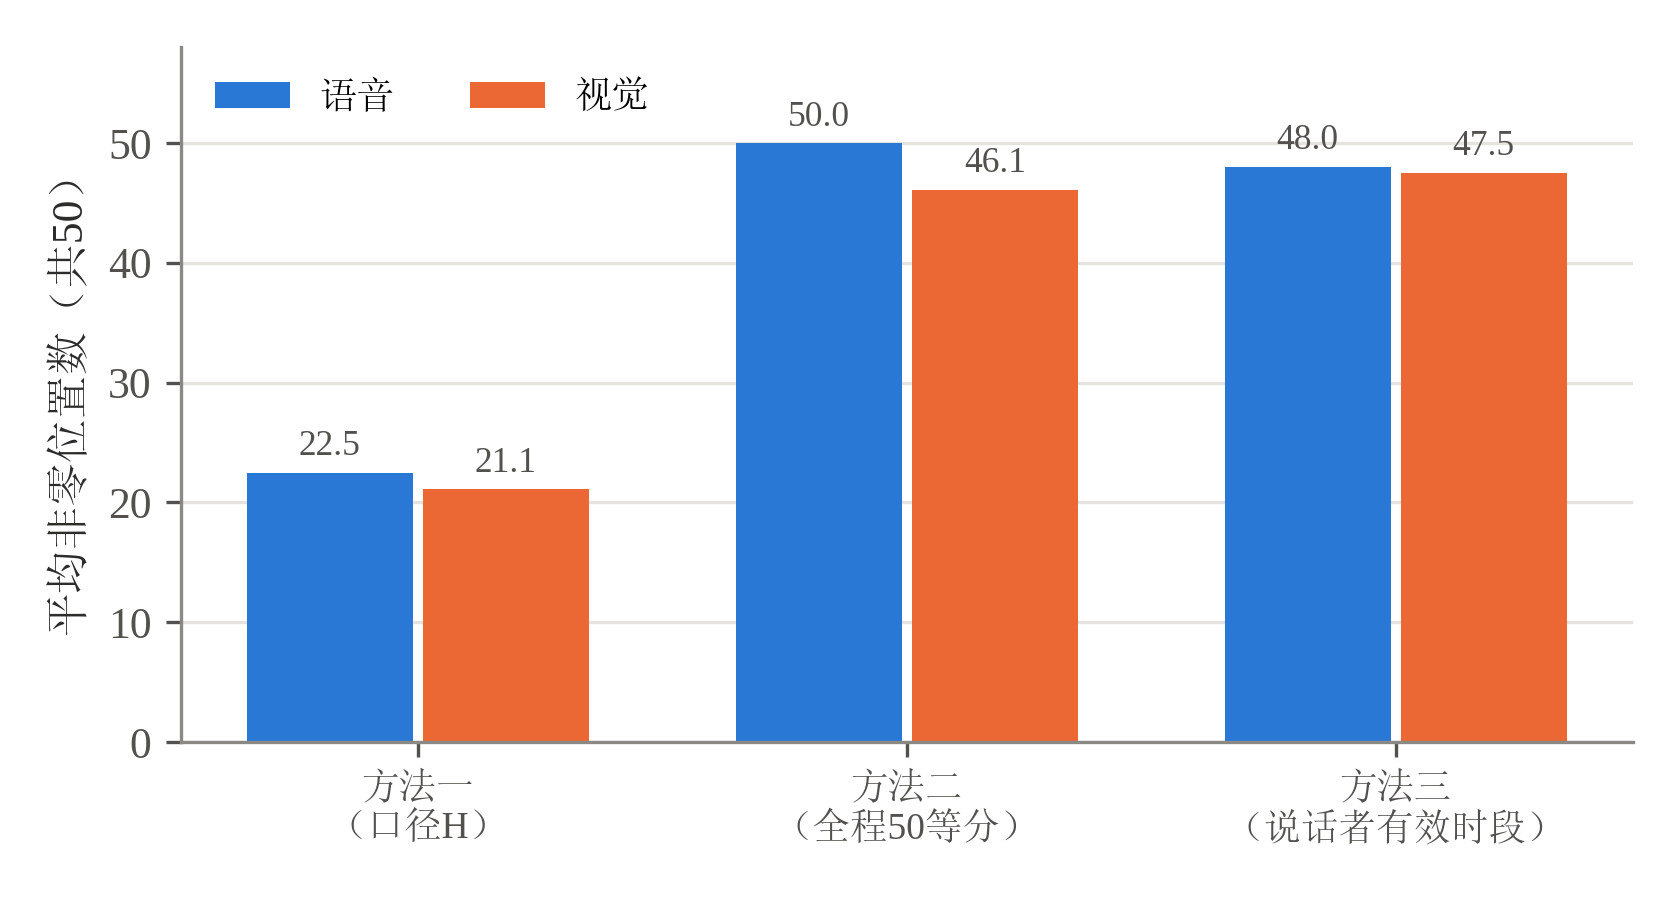
\includegraphics[width=0.72\textwidth]{figures/fig_q1_nonzero.png}
\caption{三种对齐方案下语音、视觉的平均非零位置数}
\label{fig:q1nz}
\end{figure}

方法一的语音非零位置为22.5，正好等于平均词元数减去 \texttt{[CLS]} 和 \texttt{[SEP]}（$24.5-2$），与式(\ref{eq:anchorH})的构造吻合：每个有内容的位置都对应一个词，最“干净”，信息密度最高。视觉只有21.1，比语音少1.4个，差额来自说话时恰好没检测到脸的那些词。

方法二的语音50个位置全部非零。这并不是好事：静音时段的声学特征也不是零，它被平均铺进了各个位置，混入了与情感无关的内容。

方法三剔除空白后，语音、视觉仍有48.0和47.5个非零位置，视觉还比方法二多了1.4个，说明它在保留几乎全部有效内容的同时，把位置让给了说话者可见的时段。

还有一组数字能说明为什么判据要选“说话者的脸”而不是“有没有声音”：按能量 VAD，100条片段总共777秒里只有约249秒在说话，占32\%。如果只按声音划定有效时段，三分之二的时长会被丢掉，其中包括大量不说话、但表情仍在变化的片段。按说话者脸可见来判定，平均只剪掉约7\%的时长；被剪掉的部分里，真正属于说话的只占全部语音帧的约8\%，而这些时刻视觉特征本来就缺失，剔除后反而保证了每个保留位置上三路特征都是完整的。

也要实事求是地说，在附件1上方法二和方法三的差别并不大。CMU-MOSEI 的片段大多是正对镜头的独白，说话者的脸88\%的时间都在画面里，可剔除的空白本来就少。方法三的优势在镜头切换多、人物频繁出画的视频上会更明显，这一点我们没有条件在本题数据上验证。

\subsection{典型样本验证}\label{sec:q1case}

我们选取了一条有代表性的样本：有效时长占比0.92，共30个词，含两段说话，样本编号为 \todo{样本编号}，文本为 \todo{文本片段}。图\ref{fig:q1case}最上方是音频能量包络，红色标出 VAD 判定的两段说话；下面三行依次是三种方案下 text、audio、vision 在50个位置上的非零填充模式。

\IfFileExists{figures/q1_typical_sample.png}{%
\begin{figure}[htbp]
\centering
\includegraphics[width=\textwidth]{figures/q1_typical_sample.png}
\caption{典型样本的音频能量与三种方案的特征填充模式}
\label{fig:q1case}
\end{figure}}{%
\begin{figure}[htbp]
\centering
\fbox{\parbox{0.9\textwidth}{\centering\vspace{1.5cm}\todo{把 eval/visualize\_sample.py 输出的图片重命名为 q1\_typical\_sample.png 放入 figures/ 后重新编译}\vspace{1.5cm}}}
\caption{典型样本的音频能量与三种方案的特征填充模式}
\label{fig:q1case}
\end{figure}}

从图中可以直接读出三种方案的差别：方法一只有词所在的位置非零，后面是整齐的补零；方法二把50个位置全部铺满，两段说话之间的静音也占了位置；方法三剔除了说话者不可见的时段，两段说话和其间仍在画面里的表情都得到保留。结合第\ref{sec:q1file}节的对应规则，任意一个位置都能还原到原文的词（方法一）或原视频的时刻与帧号（方法二、三），再回到视频中核对。

\subsection{可复现性说明}\label{sec:q1repro}

全部代码按方案分目录组织，每个目录内含 text\_feat.py、audio\_feat.py、vision\_feat.py、align.py 和入口 main.py，方法三另有 vad.py 与 face\_track.py；评估与可视化脚本在 eval 目录中。BERT 与 YuNet 的权重随代码包一并提供，无需另行下载。关键参数见表\ref{tab:q1param}，运行环境与命令见附录\ref{app:env}。

\begin{table}[htbp]
\centering
\caption{问题一的关键参数}
\label{tab:q1param}
\begin{tabularx}{\textwidth}{>{\raggedright\arraybackslash}p{4.4cm}>{\raggedright\arraybackslash}p{4.1cm}>{\raggedright\arraybackslash}X}
\toprule
参数 & 取值 & 说明 \\
\midrule
MAX\_POS & 50 & 统一的序列位置上限 \\
TEXT / AUDIO / VISION\_DIM & 768 / 74 / 35 & 三模态特征维度 \\
文本模型 & bert-base-uncased & 取最后一层隐状态，参数冻结 \\
音频 & 16 kHz，25 ms 窗 / 10 ms 帧移 & librosa 声学描述子 \\
视觉 & YuNet（2023mar 版 onnx），10 fps & 取面积最大的人脸 \\
对齐核 & 三角核 & 式(\ref{eq:tri}) \\
VAD\_ENERGY\_RATIO & 0.05 & 语音帧阈值为峰值短时能量的5\% \\
VAD\_MIN\_SPEECH / MAX\_GAP & 0.15 s / 0.25 s & 剔除短语音段 / 填补短静音 \\
FACE\_AREA\_RATIO（$\kappa$） & 0.4 & 说话者脸可见的面积比阈值 \\
SEED & 2026 & 随机种子 \\
\bottomrule
\end{tabularx}
\end{table}

\subsection{小结}

问题一用 BERT、librosa 和 YuNet 提取了768、74、35维的三路特征，并用同一个三角核算子给出了三种对齐方案。按词位置对齐的口径H与附件2的构造完全一致，每个位置对应一个词，可逐位回指原文；本文提出的说话者人脸跟踪方案，以“说话者的脸是否可见”划定有效时段，在100条样本上平均保留了93\%的时长，语音、视觉分别有48.0和47.5个非零位置，既剔除了无人时段，又没有丢掉不说话时的表情。

% ==================================================================
\section{附件2—4的数据核查与预处理}\label{sec:data}
% ==================================================================

从这一章起转入问题二、三。与问题一自己提取特征不同，这两问直接使用附件2—4提供的现成特征。这一章的工作看起来是准备性质的，但后来证明是整个建模过程里最关键的一步：两个问题的技术路线，都是被这里的发现改写的。

\subsection{三个附件的概况}

表\ref{tab:attach}汇总了三个附件的内容。附件2是唯一带标签的数据，模型只能在它上面训练和选型；附件3只有 BERT 的三路整数输入（词元编号、注意力掩码、分段编号），没有现成的文本特征；附件4的20条样本中有5条能按编号在附件2里精确找回，可以当作一个很小的带标签检验集。

\begin{table}[htbp]
\centering
\caption{附件2—附件4概况}
\label{tab:attach}
\begin{tabularx}{\textwidth}{cXcc}
\toprule
附件 & 内容 & 规模 & 标签 \\
\midrule
附件2 & aligned\_50.pkl：text $(50,768)$、audio $(50,74)$、vision $(50,35)$ & 4850 条 & 极性三分类 + 强度 \\
附件3 & text\_bert $(3,50)$、audio、vision & 30 条 & 无 \\
附件4 & 三模态特征 + 原始 mp4 视频 & 20 条 & 无（5条可从附件2找回） \\
\bottomrule
\end{tabularx}
\end{table}

本文采用对齐版特征 aligned\_50.pkl，训练、验证和两个专项测试集全程使用同一版本和同一输入接口。训练集共3395条样本。

\subsection{零帧结构：题目说的缺失，附件2里几乎没有}\label{sec:zero}

我们把每一帧的特征向量求 $L_2$ 范数，小于 $10^{-8}$ 的记为“全零帧”，再按零帧所在位置把它们分成四类：整条全零、尾部连续零段、起始零段、句中零段。图\ref{fig:zeromap}(a)把训练集3395条样本逐行画出来（按语音有效长度排序，深色为零帧），(b)是有效长度的累积分布。

\begin{figure}[htbp]
\centering
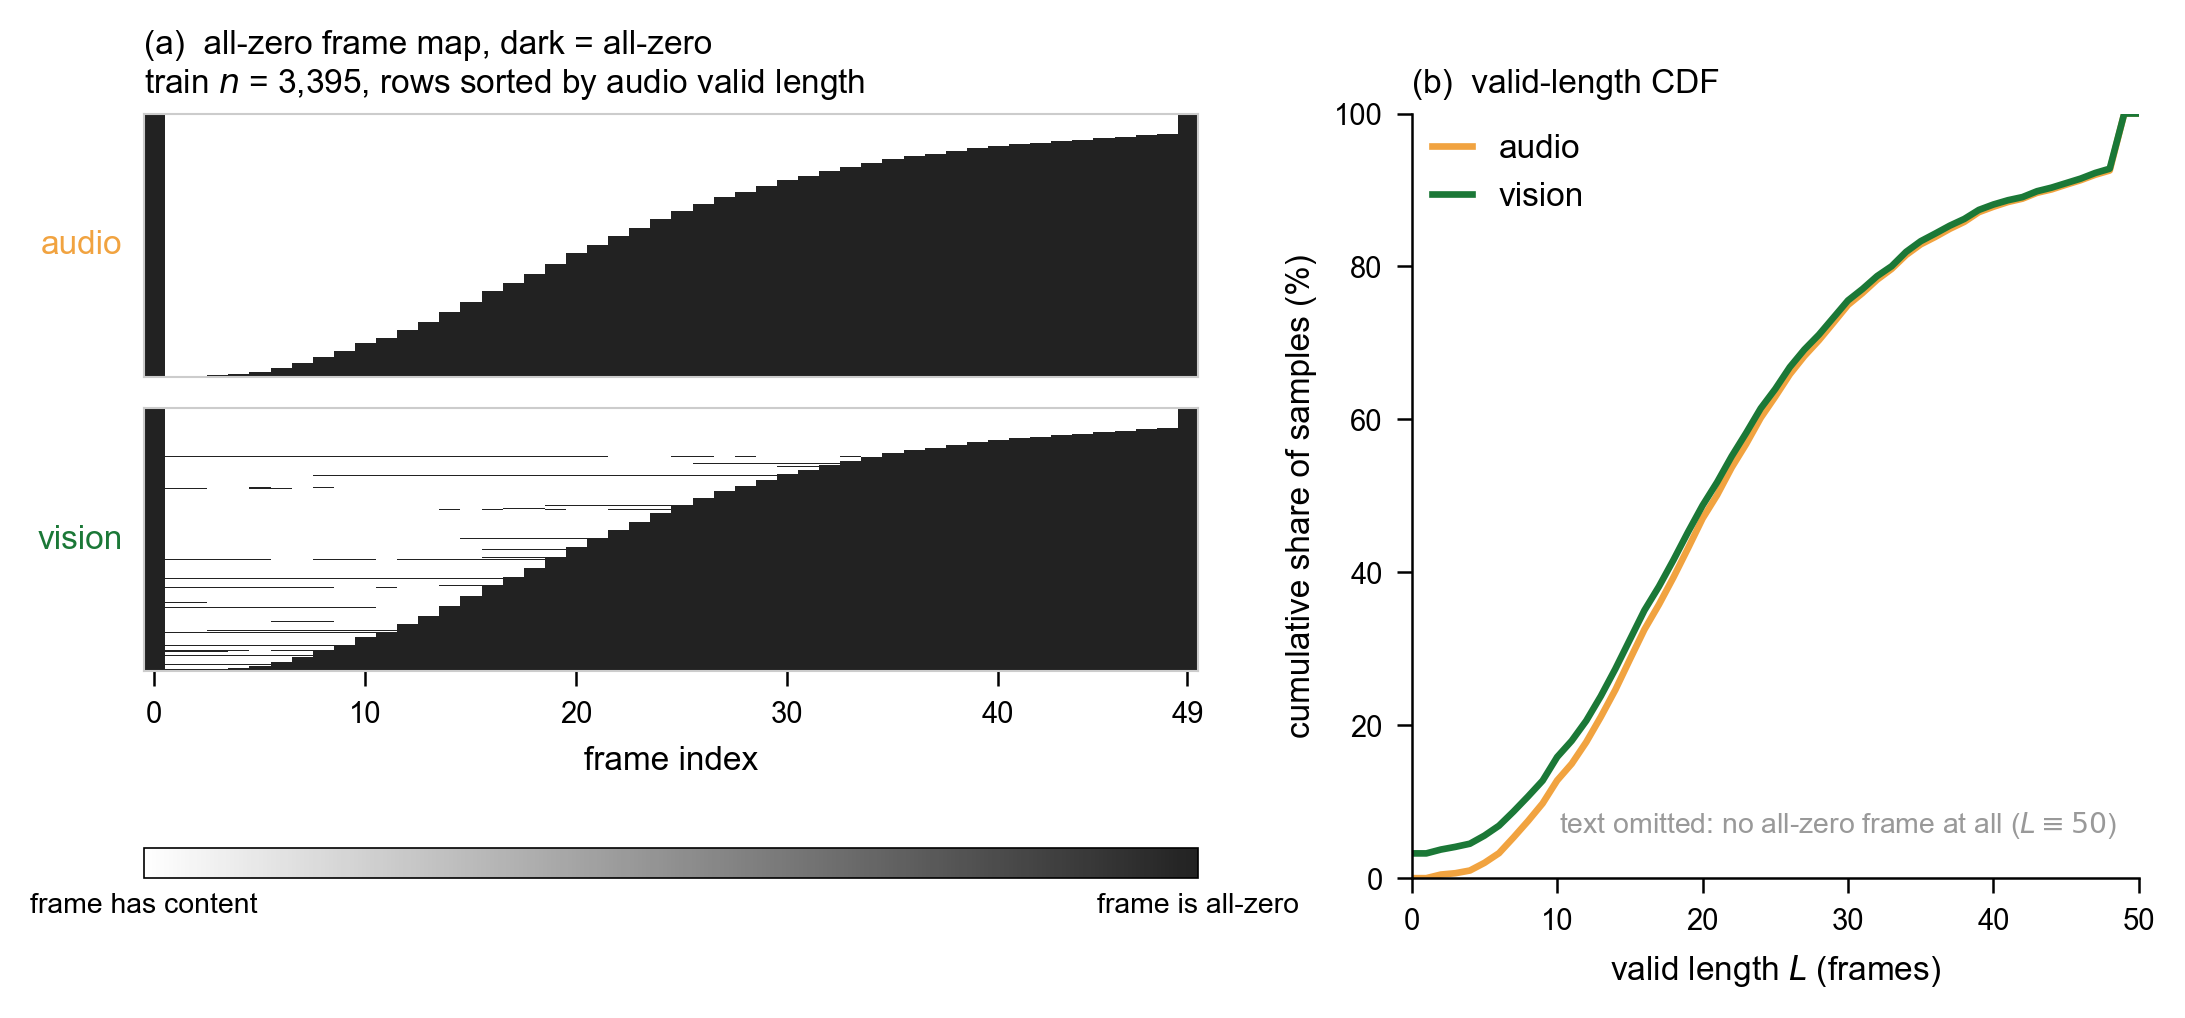
\includegraphics[width=\textwidth]{figures/fig_data_structure.png}
\caption{附件2训练集的零帧分布（a）与有效长度累积分布（b）}
\label{fig:zeromap}
\end{figure}

语音和视觉两张图的阶梯右边界几乎重合，说明两者共用同一段时间轴；文本一行深色都没有，所以没有画出来。有效长度的中位数只有21帧，也就是说一半以上的样本，后面二十多帧全是补齐用的零。表\ref{tab:zero}给出了具体统计。

\begin{table}[htbp]
\centering
\caption{附件2训练集（$N=3395$）零帧统计}
\label{tab:zero}
\begin{tabularx}{\textwidth}{lXl}
\toprule
现象 & 统计结果 & 性质 \\
\midrule
尾部连续零段 & 占零帧比例：语音 96.28\%，视觉 89.18\%；中位长度约29帧 & 变长序列补齐 \\
第0帧全零 & 语音 100\% 的样本，视觉 94\% 的样本 & 对齐产物 \\
句中连续零段 & 语音 0 段，文本 0 段；视觉 210 段（146条，4.3\%） & 零星 \\
文本零帧比例 & 0.0\%（50帧全部有值） & 无缺失 \\
\bottomrule
\end{tabularx}
\end{table}

结论很直接：题目定义的“部分连续时间段不可用”，在附件2的语音和文本上一段都不存在，视觉上也只有4.3\%的样本零星出现。附件2里所谓的连续零段，绝大多数是“这句话本来就这么长”留下的填充。附件3恰好相反，30条样本全部含句中连续缺失（语音30/30，视觉30/30），显然是人为构造的专项测试集。

这个发现改变了问题二的技术路线。如果照搬文献中的缺失设定去训练（整条模态丢弃，或者逐帧独立随机丢弃），模型面对的失效模式和附件3根本不是一回事，训练出来的“鲁棒性”是假的。图\ref{fig:missmodes}把几种形态放在一起对比：(a)是附件2的真实结构，(b)(c)是基线代码中的两种缺失模拟方式，(d)才是题目要求的连续段缺失。四种形态的总体缺失率在42.6\%到58.2\%之间，相差不大，但(b)(c)根本造不出句中的连续段。

\begin{figure}[htbp]
\centering
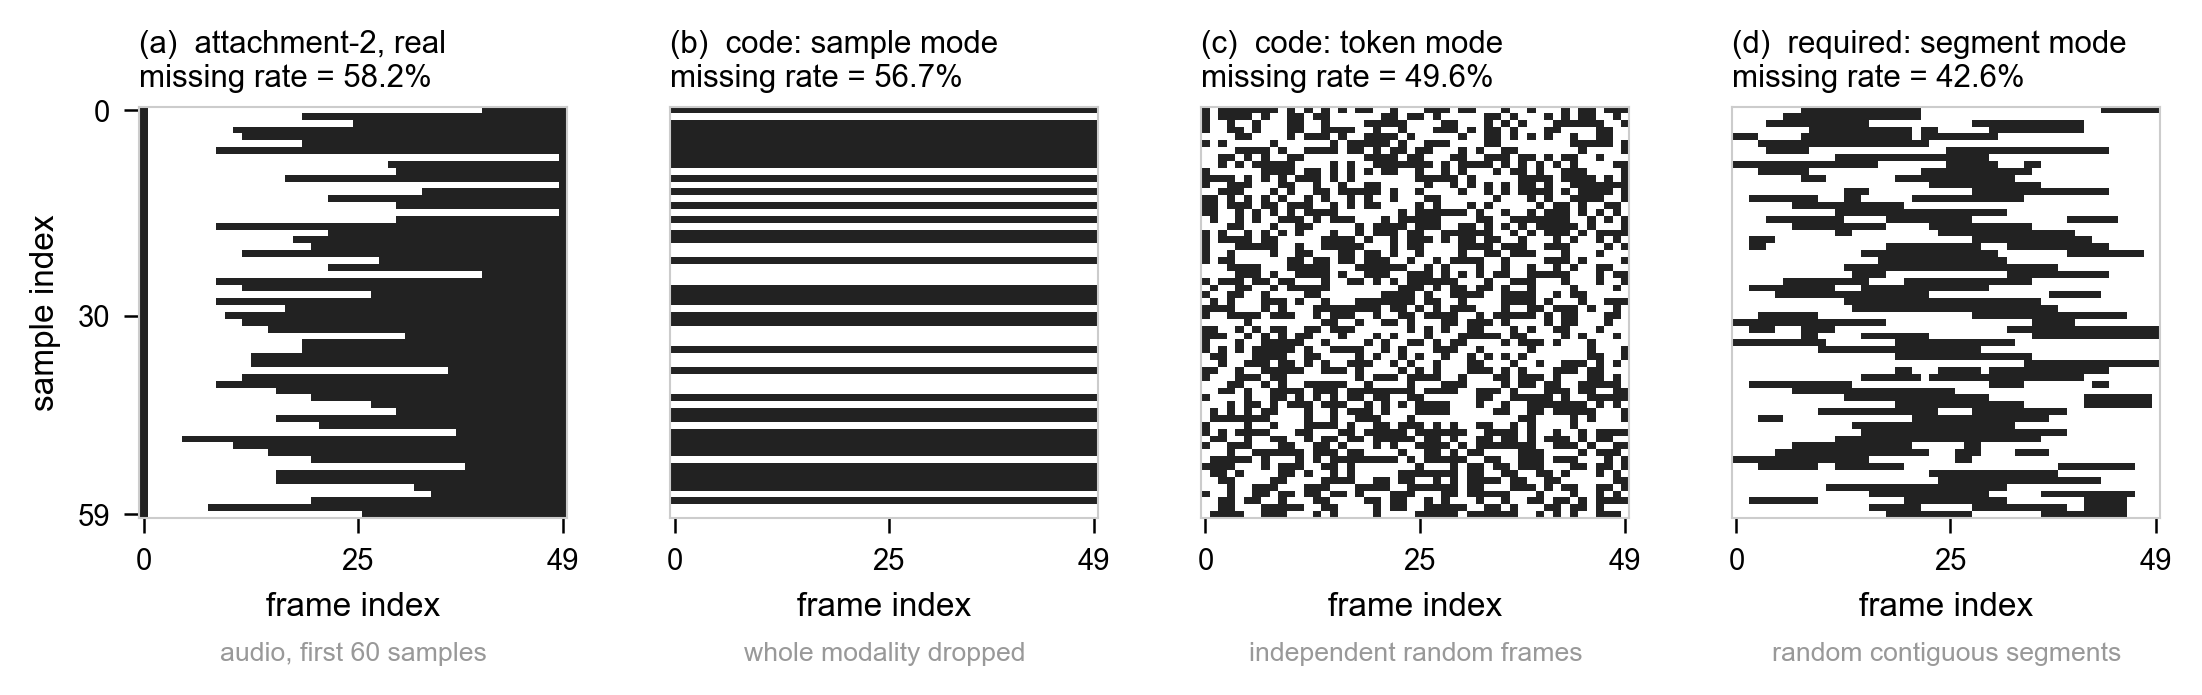
\includegraphics[width=\textwidth]{figures/fig_missing_modes.png}
\caption{缺失形态对比：(a) 附件2真实结构；(b) 整模态丢弃；(c) 逐帧独立丢弃；(d) 连续段缺失}
\label{fig:missmodes}
\end{figure}

\subsection{50个序列位置到底是什么}\label{sec:align}

问题三要求证据“能对应至原始文本片段、语音时段或视觉关键帧”，这逼着我们先弄清楚50个序列位置的物理含义。如果不知道一帧代表什么，所谓的“关键帧”就无从谈起。

如果50帧是按时间等间隔采样的，有效长度应该和片段时长相关。实测结果却是：语音有效长度与文本词元数完全线性相关，
\begin{equation}\label{eq:align}
L_a=\mathrm{nnz}(\texttt{input\_ids})-1,\qquad \mathrm{corr}\big(L_a,\ \#\mathrm{tokens}\big)=1.0000,
\end{equation}
其中 $\mathrm{nnz}(\cdot)$ 表示非零元素个数。该关系在训练、验证、测试三个划分上逐条成立，没有例外。结合 $\texttt{input\_ids}=[\,\texttt{[CLS]},w_1,\dots,w_K,\texttt{[SEP]},0,\dots]$ 的结构可知，第 $t$ 帧对应第 $t$ 个词元：第0帧对应 \texttt{[CLS]}（这也解释了为什么第0帧几乎总是全零），第 $1$ 到第 $K$ 帧依次对应句中的词元。所以这50帧不是时间采样，而是词级对齐。这与问题一中口径H的构造（式(\ref{eq:anchorH})）完全一致：第0帧为零，有效长度等于词元数减1，其后全部补零。问题一选择复刻这一口径，依据就在这里。

由此得到两条后面直接用到的结论：
\begin{enumerate}[label=(\arabic*)]
\item 文本证据可以精确回指：帧号 $\to$ 词元 $\to$ \texttt{tokenizer.decode} $\to$ 原文的词，任何一条证据都能当场人工核对。
\item 语音、视觉只能给“词级锚点”：数据里没有逐词时间戳，只能说“说第 $t$ 个词时的那段语音或表情”，给不出绝对秒数。
\end{enumerate}
对于第二条，我们也考虑过用“平均词长 $\times$ 总时长”估一个秒数，但这样得到的数字误差没法控制，恰恰违背了“可复核”的要求，所以最终只给能给准的东西。

\subsection{预处理}\label{sec:prep}

预处理共三步，做法和理由见表\ref{tab:prep}。

\begin{table}[htbp]
\centering
\caption{预处理步骤}
\label{tab:prep}
\begin{tabular}{>{\raggedright\arraybackslash}p{2.1cm}>{\raggedright\arraybackslash}p{5.6cm}>{\raggedright\arraybackslash}p{5.6cm}}
\toprule
步骤 & 做法 & 原因 \\
\midrule
有效长度提取 & 在标准化\textbf{之前}，从原始特征计算 $L_m$，见式(\ref{eq:validlen}) & 标准化后填充位置的零会变成常数向量，边界就检测不出来了 \\
标准化 & 语音、视觉用训练集统计量做 z-score，见式(\ref{eq:zscore})；文本保持 BERT 原值 & 避免信息泄漏；COVAREP\cite{degottex2014covarep} 语音特征原始值可达500，量纲差异很大 \\
文本重建 & 附件3只有词元编号，用 bert-base-uncased\cite{devlin2019bert} 现场编码 & 已验证附件2的 text 字段就是该模型的 last\_hidden\_state \\
\bottomrule
\end{tabular}
\end{table}

有效长度和标准化分别为
\begin{equation}\label{eq:validlen}
L_m=1+\max\big\{\,t:\ \|U_m^0[t]\|_2>10^{-8}\,\big\},
\end{equation}
\begin{equation}\label{eq:zscore}
\tilde U_m[t,k]=\frac{U_m^0[t,k]-\mu_{m,k}}{\sigma_{m,k}},\qquad m\in\{a,v\},
\end{equation}
其中 $\mu_{m,k}$、$\sigma_{m,k}$ 是训练集第 $k$ 维特征的均值和标准差。

表\ref{tab:prep}第一行的顺序问题是我们实际踩过的坑。最初我们先做标准化，再用标准化后的数据去算有效长度，结果零帧率从55\%一下变成了0\%，所有填充帧都“消失”了。原因就是 z-score 把全零向量变成了常数向量 $(0-\mu)/\sigma$，按范数判断就再也找不到它们。

文本重建一步也做了核对：在附件2上，用同一个 bert-base-uncased 模型对 text\_bert 字段重新编码，得到的结果与现成的 text 字段相关系数为1.0000，平均绝对差为0.0000（保留四位小数）。因此附件3重建出的文本特征与训练数据处在同一个空间里。

% ==================================================================
\section{基础模型：语言主导融合与自蒸馏}\label{sec:base}
% ==================================================================

问题二和问题三用的是同一个预测网络。这一章先把它建好：以文献\cite{shi2026ldsd}提出的 LDSD 为骨架，做两处必要的适配。问题二在此基础上改造缺失处理，问题三在它外面加解释层。

\subsection{为什么选 LDSD}

多模态情感分析的主流做法大致有两类：一类是跨模态注意力融合，如 MulT\cite{tsai2019mult}；另一类是先学模态不变与模态特有的表示再融合，如 MISA\cite{hazarika2020misa}、Self-MM\cite{yu2021selfmm}。它们大多默认三路输入完整。面向缺失的工作则多采用重建或蒸馏的思路，如 TFR-Net\cite{yuan2021tfrnet}、LNLN\cite{zhang2024lnln}。

LDSD 有两个设计正好对应本题的需要。第一是语言主导：把语言作为主模态，语音和视觉作为辅助，用语言去“查询”辅助模态中有用的部分，这一思路来自 ALMT\cite{zhang2023almt}。第\ref{sec:zero}节已经看到，附件2的文本50帧全部有值，语音、视觉则大量是填充，让信息最稠密的模态当主导是合理的。第二是自蒸馏重建：教师网络看完整输入，学生网络看缺失输入，用教师的重建结果指导学生，恰好对应“缺失下重建信息”的需求。当然，“语言主导”在本题数据上是否真的成立，不能只凭直觉，第\ref{sec:ablation}节会用两组消融专门检验。

\subsection{网络结构}

网络结构如图\ref{fig:arch}所示，下面按数据流向逐层写出。

\begin{figure}[htbp]
\centering
\begin{tikzpicture}[
  node distance=3mm,
  blk/.style={draw=black!60, rounded corners=2pt, align=flush center, font=\small, inner sep=3pt, minimum height=8mm},
  full/.style={blk, text width=13.2cm, fill=black!4},
  half/.style={blk, text width=6.3cm, minimum height=15mm},
  arr/.style={-{Stealth[length=1.8mm]}, draw=black!70, semithick}]
\node[full] (in) {输入：文本 $U_l^1$（$T\times768$），语音 $U_a^1$（$T\times74$），视觉 $U_v^1$（$T\times35$），缺失掩码 $M_a,M_v$};
\node[full, below=of in] (emb) {模态嵌入：统一到 $d=128$ 维\quad 式(\ref{eq:emb})};
\node[full, below=of emb] (lang) {语言多尺度编码：两层8头 Transformer 得到 $H_l^2,H_l^3$\quad 式(\ref{eq:lang})};
\node[full, below=of lang] (ahl) {自适应超模态学习（AHL）：以 $H_l^j$ 为 Query 聚合语音、视觉\quad 式(\ref{eq:alpha})～(\ref{eq:hyp})};
\node[full, below=of ahl, draw=red!60!black, fill=red!8, very thick] (inp) {\textbf{超模态补洞（M4，本文新增）}：在缺失帧上用 $E_{rec}(H_{Hyp})$ 替换 $H_{Hyp}$\quad 式(\ref{eq:inpaint})};
\node[half, below=6mm of inp.south west, anchor=north west, fill=black!8] (rec) {重建与自蒸馏\\ $E_{rec}(H_{Hyp}^3)\to H^{rec}$，EMA 教师 $\eta=0.99$\\ 损失 $\mathcal{L}_{rec}$\quad 式(\ref{eq:rec})～(\ref{eq:ema})};
\node[half, below=6mm of inp.south east, anchor=north east, fill=blue!5] (fus) {跨模态融合与预测\\ $H=\mathrm{CrossTrans}(H_l,H_{Hyp})$\\ 回归头 + 三分类头\quad 式(\ref{eq:fusein})～(\ref{eq:heads})};
\node[full, below=6mm of rec.south west, anchor=north west, fill=black!4] (obj) {总目标：$\mathcal{L}=\lambda\mathcal{L}_{rec}+\gamma(\mathcal{L}_{reg}+\mathcal{L}_{cls})$，$\lambda=0.5$，$\gamma=1.0$\quad 式(\ref{eq:total})};
\node[full, below=5mm of obj, dashed, fill=orange!6] (xai) {问题三解释层（不改网络）：逐模态干预、滑动窗口遮蔽、帧—词元回指};
\foreach \x/\y in {in/emb,emb/lang,lang/ahl,ahl/inp} \draw[arr] (\x) -- (\y);
\draw[arr] (inp.south -| rec.north) -- (rec.north);
\draw[arr] (inp.south -| fus.north) -- (fus.north);
\draw[arr] (rec.south) -- (rec.south |- obj.north);
\draw[arr] (fus.south) -- (fus.south |- obj.north);
\draw[arr, dashed] (obj.south) -- (xai.north);
\end{tikzpicture}
\caption{预测网络结构（红框为问题二新增的补洞模块，它与左下方的重建器共用 $E_{rec}$；虚线框为问题三的解释层）}
\label{fig:arch}
\end{figure}

\textbf{（1）模态嵌入。}三路输入维度各不相同，先各自拼接一个随机初始化、可学习的模态嵌入张量 $H_m^0$，再经线性投影和一层8头 Transformer 统一到 $d$ 维：
\begin{equation}\label{eq:emb}
H_m^1=E_m^1\big(\mathrm{concat}(H_m^0,\ U_m^1)\big)\in\mathbb{R}^{T\times d},\qquad m\in\{l,a,v\}.
\end{equation}
缺失在这一步注入：语音、视觉的缺失帧置零；语言的缺失帧替换为一个可学习的 \texttt{[UNK]} 向量（文献\cite{shi2026ldsd}用的是 BERT 的 \texttt{[UNK]} 词元，这里取它在特征空间里的等价物）。

\textbf{（2）语言多尺度编码。}语言是主模态，在 $H_l^1$ 之上再叠两层编码器，得到三个尺度：
\begin{equation}\label{eq:lang}
H_l^i=E\big(H_l^{i-1};\ \theta_{E_l}^i\big)\in\mathbb{R}^{T\times d},\qquad i\in\{2,3\}.
\end{equation}
与式(\ref{eq:emb})中把输入写进初始化张量的嵌入层不同，这两层直接对语言特征本身建模。

\textbf{（3）自适应超模态学习。}第 $j$ 层以语言第 $j$ 个尺度作 Query，从语音、视觉中聚合信息：
\begin{align}
\alpha&=\mathrm{softmax}\!\left(\frac{H_l^j W_{Q_l} W_{K_a}^{\top} H_a^{1\top}}{\sqrt{d_k}}\right),\label{eq:alpha}\\
\beta&=\mathrm{softmax}\!\left(\frac{H_l^j W_{Q_l} W_{K_v}^{\top} H_v^{1\top}}{\sqrt{d_k}}\right),\label{eq:beta}\\
H_{Hyp}^j&=H_{Hyp}^{j-1}+\alpha H_a^1 W_{V_a}+\beta H_v^1 W_{V_v},\qquad j\in\{1,2,3\},\label{eq:hyp}
\end{align}
其中 $d_k=16$，共8头。$\alpha_{t,t'}$ 的含义是“语言第 $t$ 个词在多大程度上关注语音第 $t'$ 帧”，这本身就是一条可解释线索，第\ref{sec:q3}章会用到。

\textbf{（4）重建与自蒸馏。}重建器由两层8头 Transformer 加线性输出层构成，从超模态表示中重建三个模态：
\begin{align}
H_m^{rec}&=E_{rec}\big(H_{Hyp}^3\big),\qquad m\in\{v,a,l\},\label{eq:rec}\\
H^{rec}&=\mathrm{concat}\big(H_v^{rec},H_a^{rec},H_l^{rec}\big).\label{eq:reccat}
\end{align}
教师网络接收完整输入，学生网络接收缺失输入，重建损失约束两者的重建结果一致；教师不参与梯度更新，参数由学生的指数滑动平均（EMA）得到\cite{tarvainen2017mean}：
\begin{align}
\mathcal{L}_{rec}&=\frac{1}{N_b}\sum_{n=1}^{N_b}\big\|H^{rec}_{tea,n}-H^{rec}_{stu,n}\big\|_2^2,\label{eq:lrec}\\
\theta_t^{tea}&=\eta\,\theta_{t-1}^{tea}+(1-\eta)\,\theta_t^{stu},\qquad \eta=0.99.\label{eq:ema}
\end{align}
因为教师看到的是完整输入，它的重建结果代表“信息无损时应有的样子”，比单纯的自监督重建目标更强\cite{hinton2015distilling}。

\textbf{（5）跨模态融合。}在语言和超模态序列前各拼接一个可学习的汇聚向量 $H^0$，由主导模态提供 Query、超模态提供 Key 和 Value：
\begin{align}
H_l&=\mathrm{concat}\big(H^0,H_l^3\big),\qquad H_{Hyp}=\mathrm{concat}\big(H^0,H_{Hyp}^3\big),\label{eq:fusein}\\
H&=\mathrm{CrossTrans}\big(H_l,H_{Hyp}\big)\in\mathbb{R}^{1\times d}.\label{eq:fuse}
\end{align}

\textbf{（6）预测与损失。}
\begin{align}
\hat y_{reg}&=\mathrm{regressor}(H),\qquad \hat y_{cls}=\mathrm{classifier}(H),\label{eq:heads}\\
\mathcal{L}_{reg}&=\big\|y-\hat y_{reg}\big\|_2^2,\qquad \mathcal{L}_{cls}=\mathrm{CE}\big(c,\hat y_{cls}\big),\label{eq:losses}\\
\mathcal{L}&=\lambda\,\mathcal{L}_{rec}+\gamma\,\mathcal{L}_{sp},\qquad \mathcal{L}_{sp}=\mathcal{L}_{reg}+\mathcal{L}_{cls},\qquad \lambda=0.5,\ \gamma=1.0,\label{eq:total}
\end{align}
其中 $y$ 为强度标签，$c$ 为三分类极性标签，CE 为交叉熵。

\subsection{两处适配}

复现时我们只做了两处改动，都有明确理由，没有随意调整结构。

一是增加了三分类头。原文的预测损失只有回归的均方误差，分类指标由回归输出分箱得到。但本题明确要求用准确率和 F1 评价极性，附件2又自带三分类标签，所以我们在融合表示 $H$ 之后并联了一个三分类头，见式(\ref{eq:heads})和式(\ref{eq:losses})。

二是没有实现原文实验表格中出现的“对抗学习”一项。原文第3节正文中找不到它的公式和训练细节，我们不愿意凭猜测补一个进去，因此这一项没有实现。

\subsection{评价指标}\label{sec:metrics}

极性分类用三分类准确率 Acc-3 和宏平均 F1（F1-macro），强度回归用 MAE 和皮尔逊相关系数：
\begin{gather}
\mathrm{Acc}=\frac{1}{N}\sum_{n=1}^{N}\mathbb{1}\big[\hat c_n=c_n\big],\qquad
\mathrm{F1}_{\mathrm{macro}}=\frac{1}{3}\sum_{k=1}^{3}\frac{2P_kR_k}{P_k+R_k},\label{eq:clsmetric}\\
\mathrm{MAE}=\frac{1}{N}\sum_{n=1}^{N}\big|y_n-\hat y_n\big|,\qquad
\mathrm{Corr}=\frac{\sum_n(y_n-\bar y)(\hat y_n-\bar{\hat y})}{\sqrt{\sum_n(y_n-\bar y)^2}\sqrt{\sum_n(\hat y_n-\bar{\hat y})^2}},\label{eq:regmetric}
\end{gather}
其中 $P_k$、$R_k$ 为第 $k$ 类的查准率和查全率。为了便于和文献对照，另外报告按 CMU-MOSEI 常用做法由强度值换算得到的 Acc-2、Acc-5、Acc-7。需要说明的是，F1-macro 对三类一视同仁，任何一类识别得差都会明显拉低它，比 Acc-3 更能暴露类别之间的不均衡，所以本文在比较模型时更看重 F1-macro。

% ==================================================================
\section{问题二：模态局部缺失下的鲁棒情感预测}\label{sec:q2}
% ==================================================================

这一章的顺序和我们实际推进的顺序一致：先看基线在附件2上的表现，再用鲁棒性曲线和消融找它的短板，然后针对局部连续缺失做改造，最后分析缺失规律并对附件3推理。除特别注明“验证集”的结果外，本章表格中的数值均在附件2测试集上计算，且都是全量训练（3395条训练样本、200轮）后的结果。

\subsection{基线的基础性能}\label{sec:mainres}

表\ref{tab:main}给出了复现后的基线在完整模态和整模态缺失（$r=0.5$）两种条件下的结果。

\begin{table}[htbp]
\centering
\caption{基线 LDSD 的基础性能（准确率与 F1 单位为 \%）}
\label{tab:main}
\begin{tabular}{lccccccc}
\toprule
条件 & Acc-3 & F1-macro & MAE & Corr & Acc-2 & Acc-5 & Acc-7 \\
\midrule
完整模态 & 68.78 & 60.48 & 0.6628 & 0.6722 & 74.00 & 52.41 & 44.57 \\
整模态缺失 $r=0.5$ & 58.32 & 45.80 & 0.7646 & 0.4959 & 64.10 & 46.91 & 41.54 \\
\bottomrule
\end{tabular}
\end{table}

作为参照，三分类随机猜测的准确率是33.3\%，二分类约50\%。完整模态下 Acc-2 为74.00\%，文献\cite{shi2026ldsd}报告的 Acc-2 为73.48\%，两者数据集不完全相同，不能直接比高低，但处在同一量级，说明复现是可信的。MAE 为0.6628、皮尔逊相关系数为0.6722，也都明显好于随机水平。

图\ref{fig:curve}是训练过程中验证集（$r=0.5$）上的指标变化。验证集 MAE 在第10轮左右最低（约0.72），之后逐渐上升，到第110轮前后达到约0.88，最后回落到0.80附近；Acc-3 的走势与之对应，早期约53\%，后期大致在44\%～51\%之间波动。这说明在3395条训练样本上，模型训练到中后期出现了过拟合，训练轮数还有调整空间，第\ref{sec:q2err}节会再回到这一点。

\begin{figure}[htbp]
\centering
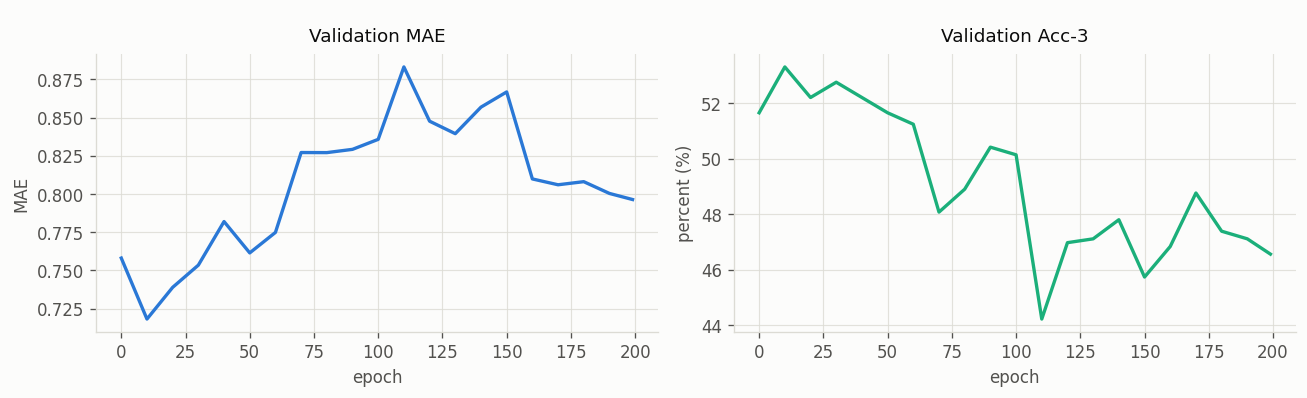
\includegraphics[width=0.92\textwidth]{figures/fig_training_curve.png}
\caption{训练过程中验证集（$r=0.5$）的 MAE（左）与 Acc-3（右）}
\label{fig:curve}
\end{figure}

\subsection{基线在整模态缺失下的鲁棒性}\label{sec:robust}

我们在整模态缺失模式下把缺失率 $r$ 从0逐步加到0.9，结果见表\ref{tab:robust}和图\ref{fig:robust}。

\begin{table}[htbp]
\centering
\caption{不同缺失率下基线的性能（整模态缺失）}
\label{tab:robust}
\begin{tabular}{lccccccc}
\toprule
$r$ & 0.0 & 0.2 & 0.4 & 0.5 & 0.6 & 0.8 & 0.9 \\
\midrule
Acc-3/\% & 68.78 & 65.47 & 62.04 & 59.56 & 56.40 & 54.33 & 50.76 \\
F1-macro/\% & 60.48 & 56.04 & 51.43 & 47.03 & 42.13 & 35.88 & 28.71 \\
MAE & 0.6628 & 0.6927 & 0.7527 & 0.7693 & 0.7750 & 0.8178 & 0.8619 \\
Corr & 0.6722 & 0.6164 & 0.5240 & 0.4883 & 0.4467 & 0.3440 & 0.2283 \\
\bottomrule
\end{tabular}
\end{table}

\begin{figure}[htbp]
\centering
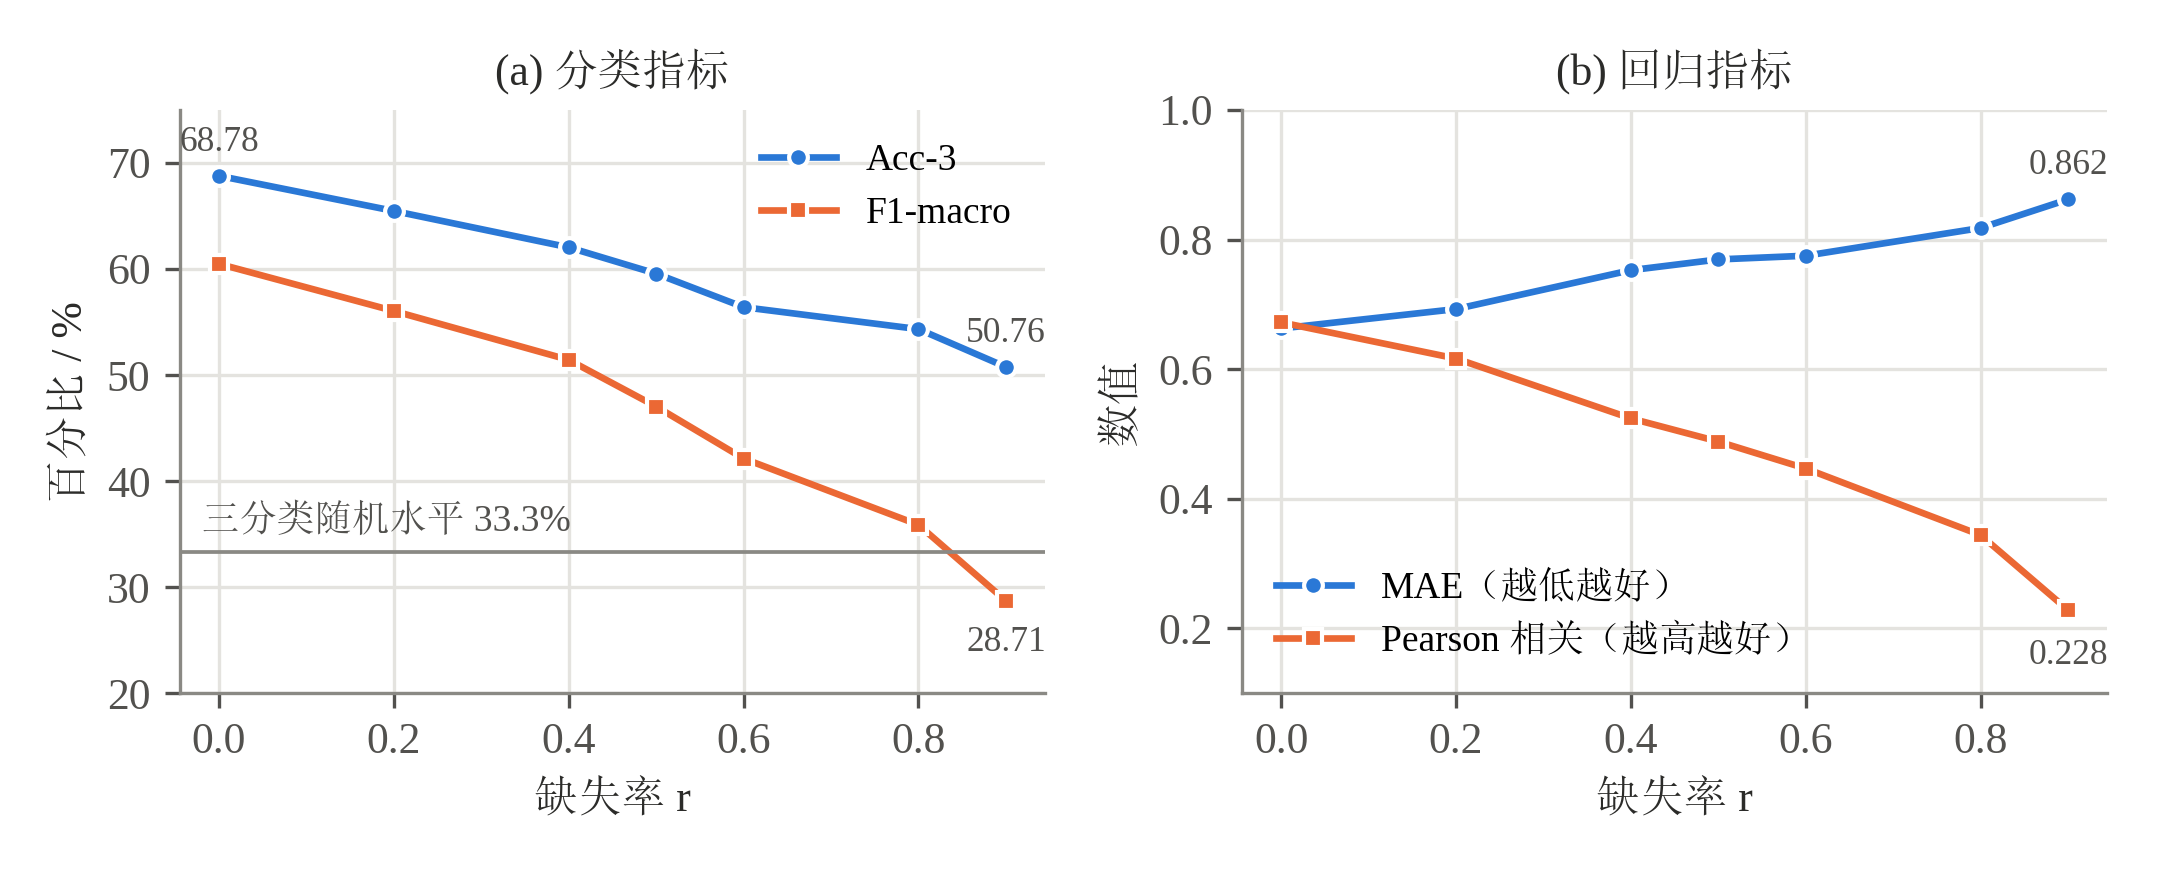
\includegraphics[width=0.95\textwidth]{figures/fig_robustness.png}
\caption{基线性能随缺失率的变化}
\label{fig:robust}
\end{figure}

整体看，性能随缺失率平滑下降，没有出现突然崩溃的拐点；即使 $r=0.9$，Acc-3 仍有50.76\%，高于随机水平。但两类指标掉得并不一样快：从 $r=0$ 到 $r=0.9$，Acc-3 下降了18.02个点，F1-macro 却下降了31.77个点，在 $r=0.9$ 时只剩28.71\%，已经低于33.3\%的随机水平。准确率还说得过去而宏平均 F1 低于随机，说明缺失严重时模型的预测集中到了少数类别上，某一类几乎不再被预测出来。这是第\ref{sec:q2err}节错误归因的第一条线索。

\subsection{三组消融：语言是不是主导，各组件有没有用}\label{sec:ablation}

LDSD 的核心主张有三条：语言不可或缺、以语言为主导模态最优、自蒸馏与重建有益。我们按这三条分别做了三组消融，每组回答一个问题，统一在 $r=0.5$ 的整模态缺失下评测。

\textbf{（1）模态消融：语言是不是不可或缺。}把某个模态的输入永久置为全缺失，并去掉它在 AHL 中的贡献，其余不变，结果见表\ref{tab:abl_mod}。

\begin{table}[htbp]
\centering
\caption{模态消融结果}
\label{tab:abl_mod}
\begin{tabular}{lccccc}
\toprule
设置 & Acc-3/\% & F1-macro/\% & MAE & Corr & F1 相对完整模型 \\
\midrule
完整模型 & 58.32 & 45.80 & 0.7646 & 0.4959 & — \\
去掉语言 & 49.79 & 22.16 & 0.8772 & 0.1620 & $-23.6$ \\
去掉语音 & 57.63 & 42.74 & 0.7643 & 0.5076 & $-3.1$ \\
去掉视觉 & 58.60 & 48.32 & 0.7578 & 0.5086 & $+2.5$ \\
\bottomrule
\end{tabular}
\end{table}

去掉语言是断崖式的：F1-macro 从45.80\%跌到22.16\%，皮尔逊相关从0.4959掉到0.1620，模型几乎失去了与人工标注的相关性。去掉语音或视觉的影响则温和得多，去掉视觉后 F1 甚至略有上升，不过幅度在正常波动范围内。

这组结果不是可有可无的对比。整个网络建立在“语言主导”的前提上，式(\ref{eq:alpha})～(\ref{eq:hyp})和式(\ref{eq:fuse})都让语言当 Query。如果去掉语言影响不大，那就说明前提是错的，后面所有围绕语言设计的模块都失去了依据。

\textbf{（2）主导模态消融：让语言当主导是不是最好的选择。}上一组只说明了语言“不能少”，没有说明“让它当主导最好”。万一让语音主导效果更好呢？所以我们把主导模态分别换成语音和视觉，即让该模态走三尺度编码、充当融合层的 Query，另外两个模态充当超模态，结果见表\ref{tab:abl_dom}。

\begin{table}[htbp]
\centering
\caption{主导模态消融结果}
\label{tab:abl_dom}
\begin{tabular}{lcccc}
\toprule
主导模态 & Acc-3/\% & F1-macro/\% & MAE & Corr \\
\midrule
语言 & \textbf{58.32} & \textbf{45.80} & \textbf{0.7646} & \textbf{0.4959} \\
语音 & 57.08 & 43.40 & 0.7736 & 0.4673 \\
视觉 & 56.67 & 45.04 & 0.7697 & 0.4744 \\
\bottomrule
\end{tabular}
\end{table}

语言主导在四项指标上全部最优。语音主导时 F1 低2.4个点、相关系数低0.029；视觉主导时 Acc-3 低1.7个点。两组合起来，才完整支撑了“语言主导”这个设计：第一组说明语言必要，第二组说明把主导权交给语言是最好的安排。

\textbf{（3）组件消融：自蒸馏和重建到底有没有用。}逐个去掉四个组件，保持其余结构不变，结果见表\ref{tab:abl_comp}。

\begin{table}[htbp]
\centering
\caption{组件消融结果}
\label{tab:abl_comp}
\begin{tabular}{lccccl}
\toprule
设置 & Acc-3/\% & F1-macro/\% & MAE & Corr & 判断 \\
\midrule
完整模型 & 58.32 & 45.80 & 0.7646 & 0.4959 & 基准 \\
去掉自蒸馏 & 56.26 & 37.48 & 0.8085 & 0.4639 & 明显退化 \\
去掉超模态融合 & 57.91 & 43.34 & 0.7772 & 0.4695 & 退化 \\
去掉重建 & 56.95 & 47.16 & 0.7538 & 0.5058 & F1、MAE 反而略好 \\
去掉 AHL & 58.32 & 46.69 & 0.7441 & 0.5098 & MAE、Corr 反而略好 \\
\bottomrule
\end{tabular}
\end{table}

结果要分两层看。正面的一层：去掉自蒸馏后 F1 下降8.3个点、MAE 上升0.044，是四个组件里影响最大的；去掉超模态融合也明显退化。这说明 EMA 教师提供的重建目标确实比单纯的自监督目标更有用，跨模态融合也是有效的。

反直觉的一层：去掉重建（MAE 0.7538）和去掉 AHL（MAE 0.7441）之后，MAE 和相关系数反而比完整模型略好。也就是说，原文“重建有益”的结论在本题数据上只得到了部分复现。我们如实报告这个结果，因为它本身有信息量。我们的理解是：在整模态缺失的设定下，一整路信号都没了，重建目标高度不确定，重建头学到的更像是一种“均值式”的补偿，反而冲淡了判别信号；去掉 AHL 后 MAE 更好，则说明样本级缺失时，AHL 学到的注意力权重可能引入了噪声。

这组结果直接推动了我们后面的两个决定。一是把训练时的缺失模拟改成连续段形态：整模态缺失下这两个模块表现不稳，恰恰说明“缺失的形态”很关键。二是让重建结果真正进入推理路径：如果重建只是算一个损失就被丢掉，它学不到有用的东西也就不奇怪了。第\ref{sec:m4}节的 M4 就是这样来的。

\subsection{面向局部连续缺失的改进}\label{sec:improve}

\subsubsection{缺失的形式化}\label{sec:missdef}

用掩码 $M_m\in\{0,1\}^T$ 描述模态 $m$ 的缺失，$M_m[t]=1$ 表示第 $t$ 帧不可用。注入缺失后，语音和视觉按 $U_m^1=U_m^0\odot(1-M_m)$ 置零，语言的缺失帧替换为可学习的 \texttt{[UNK]} 向量。按掩码的生成方式，可以区分三种缺失模式：
\begin{equation}\label{eq:modes}
M_m[t]=\begin{cases}
b_m,\quad b_m\sim\mathrm{Bernoulli}(r), & \text{整模态丢弃（sample）},\\[2pt]
b_{m,t},\quad b_{m,t}\overset{\text{i.i.d.}}{\sim}\mathrm{Bernoulli}(r), & \text{逐帧独立丢弃（token）},\\[2pt]
\mathbb{1}\big[t\in\mathcal{M}_m\big],\quad \mathcal{M}_m\ \text{为若干连续区间之并}, & \text{连续段缺失（segment）}.
\end{cases}
\end{equation}
前两种是基线代码实际使用的模式，第三种才是附件3中的形态。三种模式下 $r$ 的含义不同：整模态模式中是一个模态被整条丢弃的概率，后两种模式中是缺失帧所占的比例。

\subsubsection{M1：连续段缺失增强}

文献\cite{shi2026ldsd}第3.2节的文字描述是“随机遮蔽片段”（randomly masking segments），但我们阅读其公开代码后发现，实际实现是逐帧独立的伯努利采样，与“连续段”并不是一回事。这个差别在散点缺失下看不出来，换成连续段就会暴露（见第\ref{sec:screen}节，相差9.4个点）。因此我们显式构造连续段：
\begin{equation}\label{eq:m1}
\begin{gathered}
(\rho_1,\dots,\rho_k)\sim\mathrm{Dirichlet}(0.6\cdot\mathbf{1}_k),\qquad
\ell_j=\max\big(1,\ \lfloor\rho_j\, rT\rfloor\big),\\
\mathcal{M}_m=\bigcup_{j=1}^{k}\big[a_j,\ a_j+\ell_j\big),
\end{gathered}
\end{equation}
其中段数 $k\sim\mathcal{U}\{1,2,3\}$，$\ell_j$ 为第 $j$ 段的长度，各段在互不相交的区块内选取起点 $a_j$。

用 Dirichlet 分布分配段长，是为了让段长有足够的区分度：短段可以借邻域插值补回来，长段不行；如果生成的段长都差不多，评测时按段长分桶就看不出差异。这一点我们在调试阶段实际吃过亏：第一版的段长分布没有调好，93\%的样本都落进了“长段”桶，分桶结果什么也说明不了。最终浓度参数取0.6：浓度小于1时，各段分到的长度差异更大，更容易同时产生很短和很长的缺失段。

\subsubsection{M4：超模态补洞}\label{sec:m4}

文献\cite{shi2026ldsd}第3.1节的概述中说重建出的模态特征被用于语言主导的预测，但从其式(6)～(8)看，重建结果只参与了 $\mathcal{L}_{rec}$ 的计算，并没有进入推理路径。对连续段缺失来说，这个区别是决定性的：模型必须在洞里显式地填入推断出的表征，而不能指望下游模块自己学会忽略这个洞。因此我们补上这条通路：
\begin{equation}\label{eq:inpaint}
H_{Hyp}\leftarrow H_{Hyp}\odot(1-m)+E_{rec}\big(H_{Hyp}\big)\odot m,\qquad m=\max\big(M_a,M_v\big),
\end{equation}
即在语音或视觉任一模态缺失的帧上，用重建器的输出替换超模态表示，其余帧保持不变。这样重建器一方面仍受式(\ref{eq:lrec})的自蒸馏监督，另一方面它的输出直接影响预测，梯度会把“补得像不像”和“预测得准不准”绑在一起。

\subsubsection{其余三个候选模块}

除 M1 和 M4 外，我们还准备了另外三个候选，思路都是“让模型知道哪里缺了”：
\begin{itemize}
\item \textbf{M2 有效性 token}：为“缺失”和“填充”两种状态各设一个可学习向量，叠加到对应帧上，让模型能区分“本来没有”和“丢了”。
\item \textbf{M3 掩码加权损失}：把式(\ref{eq:lrec})的重建损失限制在缺失位置上计算，想让重建头把力气用在洞上。
\item \textbf{M5 掩码注意力}：在 AHL 的式(\ref{eq:alpha})(\ref{eq:beta})中屏蔽缺失帧对应的 Key/Value。
\end{itemize}
这五个模块哪个有用，我们事先并没有把握，所以决定全部实现，用数据决定去留。

\subsection{候选模块的逐级筛选}\label{sec:screen}

\textbf{筛选规则。}把模块逐个叠加上去，每加一个就与当前最好的配置比较一次边际增益；没有增益或者有损就淘汰，下一个模块仍然叠加在最后一个有效配置上。

\textbf{评测掩码。}所有配置统一用一套固定的分层连续段掩码评测：短段（最长缺失段 $\le5$ 帧）占40\%、中段（6～15帧）占35\%、长段（$>15$帧）占25\%。所有配置共用同一套掩码，并按样本中最长缺失段的长度分桶统计，这样不同配置之间才可比。评价时同时看三个量：段缺失下的 F1-macro、长段缺失下的 MAE，以及完整模态下的 F1-macro（用来确认改进没有伤害完整输入时的表现）。

先看 M1 单独的作用（表\ref{tab:m1}）。这组实验只改训练时的缺失模拟方式，把逐帧散点换成连续段，其余完全不变。

\begin{table}[htbp]
\centering
\caption{连续段缺失增强（M1）的作用}
\label{tab:m1}
\begin{tabular}{lccc}
\toprule
配置 & 段缺失 F1-macro/\% & 长段 MAE & 完整模态 F1-macro/\% \\
\midrule
基线（逐帧散点训练） & 47.63 & 0.7168 & 56.65 \\
+M1（连续段训练） & \textbf{57.03} & \textbf{0.6666} & \textbf{57.65} \\
\bottomrule
\end{tabular}
\end{table}

仅仅改变训练时的缺失模拟方式，段缺失 F1 就提升了9.4个点，长段 MAE 下降0.050，完整模态下的 F1 也没有退化（56.65\%$\to$57.65\%）。这证实了我们一开始的判断：连续段缺失和散点缺失是两种不同的失效模式，模型必须专门见过才会应对。而且 M1 不改网络结构，只改训练数据的构造方式，是性价比最高的一项。

接着在 M1 之上逐个叠加其余四个模块，结果见表\ref{tab:screen}和图\ref{fig:screen}。

\begin{table}[htbp]
\centering
\caption{候选模块逐级筛选结果}
\label{tab:screen}
\begin{tabular}{lcccl}
\toprule
配置 & 段缺失 F1/\% & 长段 MAE & 完整模态 F1/\% & 结论 \\
\midrule
M1（参照） & 57.03 & 0.6666 & 57.65 & 基准 \\
M1+M2 & 57.25 & 0.6702 & 57.92 & 增益在噪声内，淘汰 \\
M1+M3 & 56.37 & 0.6865 & 56.92 & 有害，淘汰 \\
M1+M4 & \textbf{60.21} & \textbf{0.6572} & \textbf{60.86} & 保留 \\
M1+M4+M5 & 58.02 & 0.6708 & 56.81 & 有害，淘汰 \\
\bottomrule
\end{tabular}
\end{table}

\begin{figure}[htbp]
\centering
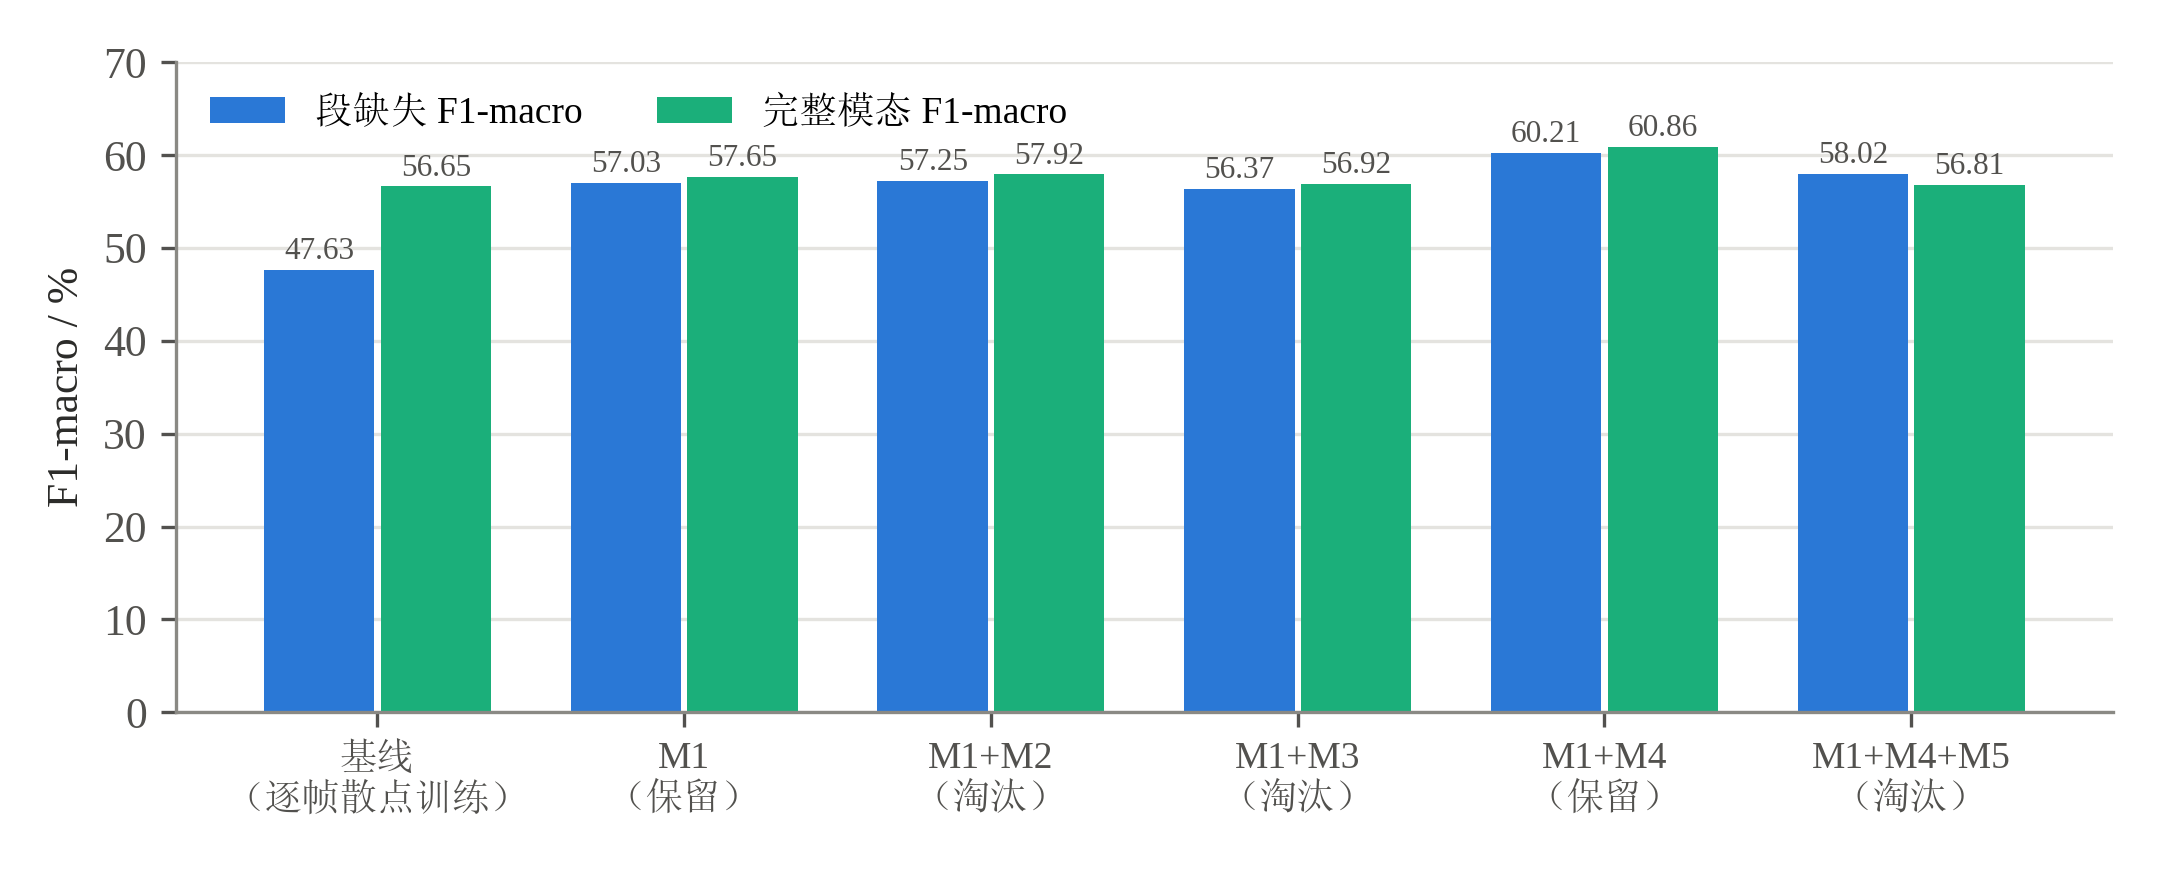
\includegraphics[width=0.95\textwidth]{figures/fig_module_screen.png}
\caption{候选模块筛选过程中段缺失与完整模态下的 F1-macro}
\label{fig:screen}
\end{figure}

只有 M4 带来了实质增益：段缺失 F1 提升3.2个点，完整模态 F1 同步提升3.2个点，长段 MAE 下降0.009。其余三个都没有通过：

M2 的 F1 只比参照高0.22个点，长段 MAE 反而从0.6666变差到0.6702，这点增益在噪声范围内，不足以成为保留的理由。

M3 明确有害。事后分析原因：把重建损失限制到缺失位置后，监督信号变得很稀疏，重建头在观测帧上失去了约束，开始“漂移”。本想让损失更聚焦，结果削弱了整体约束。

M5 同样有害。屏蔽掉大量 Key/Value 之后，注意力可用的上下文反而变少了，完整模态 F1 和长段 MAE 都比 M1+M4 差。

这里有一个流程上的教训值得单独记下。M3 判定失败时，我们原先已经把 M4、M5 叠在“M1+M3”这个坏配置上跑了一轮，那一轮结果完全不可用，只好回到最后一个有效配置 M1 上重跑，才判定出 M4 有效。如果省掉这次重跑，M4 的增益会被 M3 的损害掩盖掉，很可能被误判为无效。

回头看这组筛选，M2 和 M5 都是在给模型提供“哪里缺了”的额外信息，但都没用；真正起作用的 M4 不只是告诉模型洞在哪，而是直接把洞填上。最终保留 M1 与 M4，记为 LDSD-Seg。

\subsection{训练方案与关键参数}

表\ref{tab:params}列出了 LDSD-Seg 的主要配置。结构参数与文献\cite{shi2026ldsd}保持一致，缺失相关的参数由第\ref{sec:screen}节的筛选确定。

\begin{table}[htbp]
\centering
\caption{LDSD-Seg 的训练方案与关键参数}
\label{tab:params}
\begin{tabular}{>{\raggedright\arraybackslash}p{3.6cm}>{\raggedright\arraybackslash}p{9.2cm}}
\toprule
项目 & 设置 \\
\midrule
训练数据 & 附件2 aligned\_50.pkl 训练集3395条；验证集用于选择结构与阈值 \\
序列与维度 & $T=50$，$d=128$，8头注意力，$d_k=16$ \\
语言多尺度编码 & 在 $H_l^1$ 上叠加两层8头 Transformer \\
重建器 $E_{rec}$ & 两层8头 Transformer + 线性输出层 \\
自蒸馏 & 教师为学生参数的 EMA，$\eta=0.99$ \\
损失权重 & $\lambda=0.5$，$\gamma=1.0$，$\mathcal{L}_{sp}=\mathcal{L}_{reg}+\mathcal{L}_{cls}$ \\
缺失增强（M1） & 段数 $k\sim\mathcal{U}\{1,2,3\}$，段长按 Dirichlet$(0.6)$ 分配 \\
补洞（M4） & $m=\max(M_a,M_v)$，见式(\ref{eq:inpaint}) \\
训练轮数 & 200轮 \\
优化器、学习率、批大小 & \todo{从配置文件抄录} \\
运行环境与耗时 & Kaggle GPU；全部实验总耗时 7772.6 s（约2.16 h） \\
\bottomrule
\end{tabular}
\end{table}

\subsection{LDSD-Seg 的全量确认}\label{sec:segconfirm}

筛选阶段的结论要在最终配置上再确认一次。我们把基线（整模态缺失增强，无补洞）与 LDSD-Seg 放在同一套固定分层连续段掩码下评测。用同一套掩码是关键，否则两者面对的缺失样本不同，数字没法比。结果见表\ref{tab:seg}和图\ref{fig:seg}。

\begin{table}[htbp]
\centering
\caption{局部连续缺失下基线与 LDSD-Seg 的对比}
\label{tab:seg}
\begin{tabular}{lcccccc}
\toprule
\multirow{2}{*}{配置} & \multicolumn{3}{c}{段缺失（整体）} & \multicolumn{3}{c}{按最长缺失段分桶的 MAE} \\
\cmidrule(lr){2-4}\cmidrule(lr){5-7}
 & MAE & F1/\% & Acc-3/\% & 短段 & 中段 & 长段 \\
\midrule
基线 LDSD & 0.7112 & 47.26 & 63.82 & 0.6780 & 0.7034 & 0.7205 \\
LDSD-Seg & \textbf{0.6639} & \textbf{61.70} & \textbf{67.81} & \textbf{0.6175} & \textbf{0.6849} & \textbf{0.6548} \\
变化量 & $-0.047$ & $+14.4$ & $+4.0$ & $-0.061$ & $-0.019$ & $-0.066$ \\
\bottomrule
\end{tabular}
\end{table}

\begin{figure}[htbp]
\centering
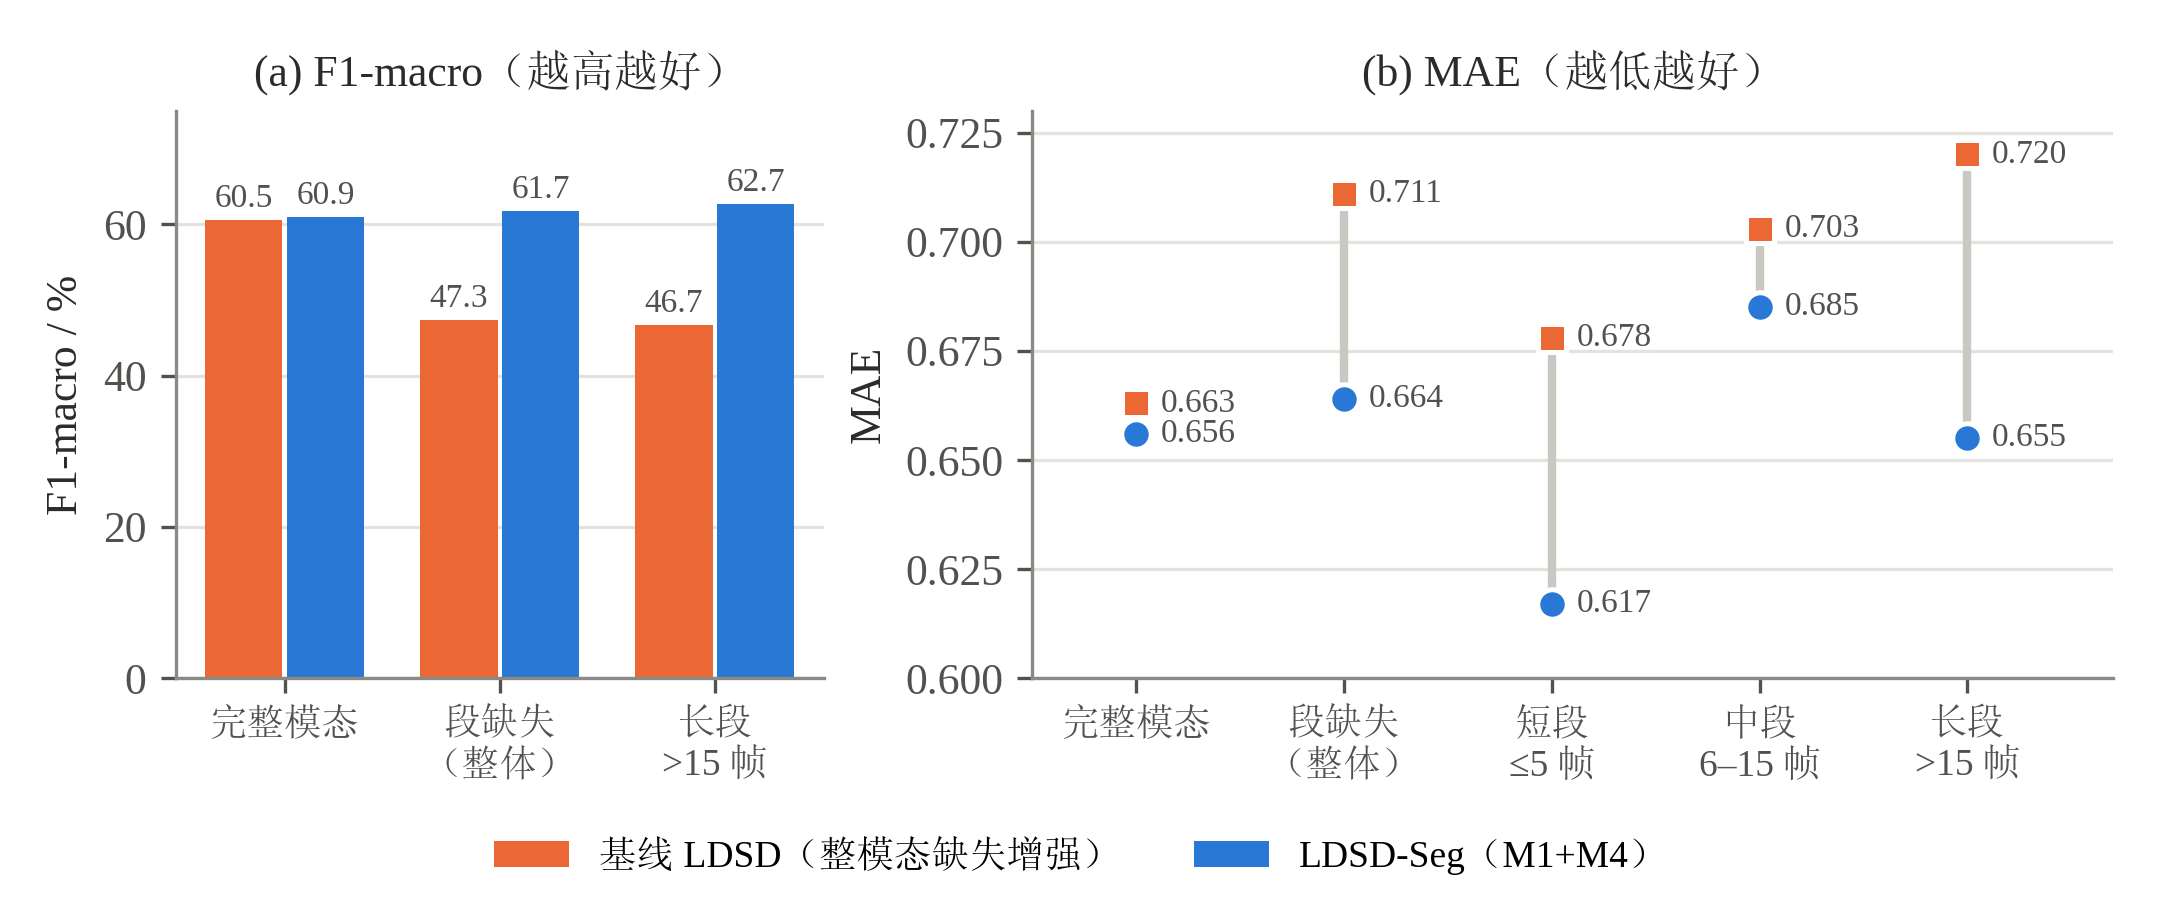
\includegraphics[width=0.95\textwidth]{figures/fig_segment_compare.png}
\caption{同一套分层连续段掩码下，基线与 LDSD-Seg 的 F1-macro（a）和 MAE（b）}
\label{fig:seg}
\end{figure}

段缺失 F1 从47.26\%提升到61.70\%，MAE 从0.7112降到0.6639。分桶看，长段 MAE 的降幅（0.066）大于整体（0.047），说明改进确实作用在最难的情形上，而不是靠容易的样本刷分。不过中段的改善最小，只有0.019，这一点我们目前还没有找到令人满意的解释，只能如实列出。

比起绝对性能，“缺失让性能掉了多少”更能说明鲁棒性。表\ref{tab:gap}是验证集上完整模态与段缺失之间的落差。

\begin{table}[htbp]
\centering
\caption{验证集上完整模态与段缺失之间的 F1-macro 落差}
\label{tab:gap}
\begin{tabular}{lccc}
\toprule
模型 & 完整模态 F1/\% & 段缺失 F1/\% & 落差 \\
\midrule
基线 LDSD & 55.56 & 39.93 & $-15.6$ \\
LDSD-Seg & 59.36 & \textbf{59.47} & $+0.1$ \\
\bottomrule
\end{tabular}
\end{table}

基线一遇到连续段缺失就掉15.6个点，LDSD-Seg 在同样条件下几乎不掉（$+0.1$，在波动范围内）。我们最初的动机只是“题目要求处理局部缺失”，但真正让我们决定保留这两个模块的依据是这个落差：它比绝对性能更直接地反映了鲁棒性有没有真的改善。

还要说明一点：同一个 M1+M4 配置，在筛选实验中段缺失 F1 为60.21\%，在这里为61.70\%，两次运行相差约1.5个点。这提示单次运行的结果存在一定波动，表中小于1个点左右的差异不宜过度解读。

\subsection{缺失类型、位置与时长的影响规律}\label{sec:factor}

\subsubsection{实验设计}

题目要求分析缺失模态类型、缺失位置、缺失时长对性能的影响。我们做了三因子扫描：
\begin{itemize}
\item 模态类型：$\{l,a,v\}$ 的6个非空真子集，即 $l$、$a$、$v$、$l{+}a$、$l{+}v$、$a{+}v$；
\item 位置：缺失段位于内容的前部（head）、中部（mid）、尾部（tail）；
\item 时长：$\rho\in\{0.10,0.25,0.50,0.75,0.90,1.00\}$，$\rho$ 为缺失段占该模态自身内容跨度的比例。
\end{itemize}
共 $6\times3\times6=108$ 个单元。模型固定为训练好的 LDSD-Seg，只训练一次，所有因子组合都只在评测时构造掩码、重新跑前向，因此108个单元不需要训练108次，扫描本身只占全部耗时的1～2分钟。指标为相对完整模态的 MAE 增量 $\Delta\mathrm{MAE}$。

\subsubsection{设计中修正的两处错误}

这两处错误都是靠事先设置的校验项抓出来的，这里单独交代一下。

\textbf{位置不能用绝对帧号。}我们最初统一用语音的有效长度 $L_a$ 来划分所有模态的前、中、尾部。结果对文本来说只遮蔽了前21帧左右，剩下的帧照样能读出情感，实测文本缺失的 $\Delta\mathrm{MAE}$ 竟然是负的，差点得出“语言缺失无害”这个完全错误的结论。正确做法是每个模态按自身的内容跨度取相对坐标。

\textbf{$\rho$ 必须铺到1.0。}各模态的冗余度不同，同一个 $\rho$ 下的绝对损失量不可比。第一版的时长只取到0.75，什么规律都看不出来；把范围扩展到0.90和1.00后，规律才显现出来。

\subsubsection{校验：语言全缺时必须最差}

在进入正式分析之前，先在 $\rho=1.0$（整模态全部遮蔽）上做一次校验，记为 H1：既然第\ref{sec:ablation}节已经证明语言不可或缺，那么语言全缺时的损失理应最大。结果见表\ref{tab:h1}。

\begin{table}[htbp]
\centering
\caption{校验 H1：$\rho=1.0$ 时各模态组合缺失的 $\Delta\mathrm{MAE}$}
\label{tab:h1}
\begin{tabular}{lcccccc}
\toprule
缺失模态 & $l$ & $l{+}a$ & $l{+}v$ & $a$ & $v$ & $a{+}v$ \\
\midrule
$\Delta\mathrm{MAE}$ & $+0.789$ & $+0.764$ & $+0.752$ & $+0.003$ & $+0.004$ & $+0.006$ \\
\bottomrule
\end{tabular}
\end{table}

语言缺失的 $\Delta\mathrm{MAE}$ 约为语音、视觉的200倍（0.789对0.004），校验成立。这组数不算新发现，它和模态消融的结论一致，本就在预料之中。它的作用是检查扫描代码有没有写对：如果这里语言不是最差的，就说明坐标定义或掩码构造有 bug。事实证明这个担心不多余，上一小节的两处错误，都是因为这项校验不成立才被发现的。因子扫描是新写的代码，一旦实现有误，错误的结论就会被当成“发现”写进报告，所以我们先设了一个已知答案的检查项。

\subsubsection{时长的影响}

表\ref{tab:dur}给出了时长的主效应及其在各模态上的分解，图\ref{fig:factor}是对应的曲线。

\begin{table}[htbp]
\centering
\caption{不同缺失时长下的 $\Delta\mathrm{MAE}$}
\label{tab:dur}
\begin{tabular}{lcccccc}
\toprule
$\rho$ & 0.10 & 0.25 & 0.50 & 0.75 & 0.90 & 1.00 \\
\midrule
全部模态平均 & $+0.003$ & $+0.005$ & $+0.008$ & $+0.016$ & $+0.033$ & $+0.386$ \\
语言 $l$ & $+0.005$ & $+0.008$ & $+0.012$ & $+0.027$ & $+0.060$ & $+0.789$ \\
语音 $a$ & $+0.001$ & $+0.001$ & $+0.002$ & $+0.003$ & $+0.003$ & $+0.003$ \\
视觉 $v$ & $+0.000$ & $+0.001$ & $+0.000$ & $+0.000$ & $+0.000$ & $+0.004$ \\
\bottomrule
\end{tabular}
\end{table}

\begin{figure}[htbp]
\centering
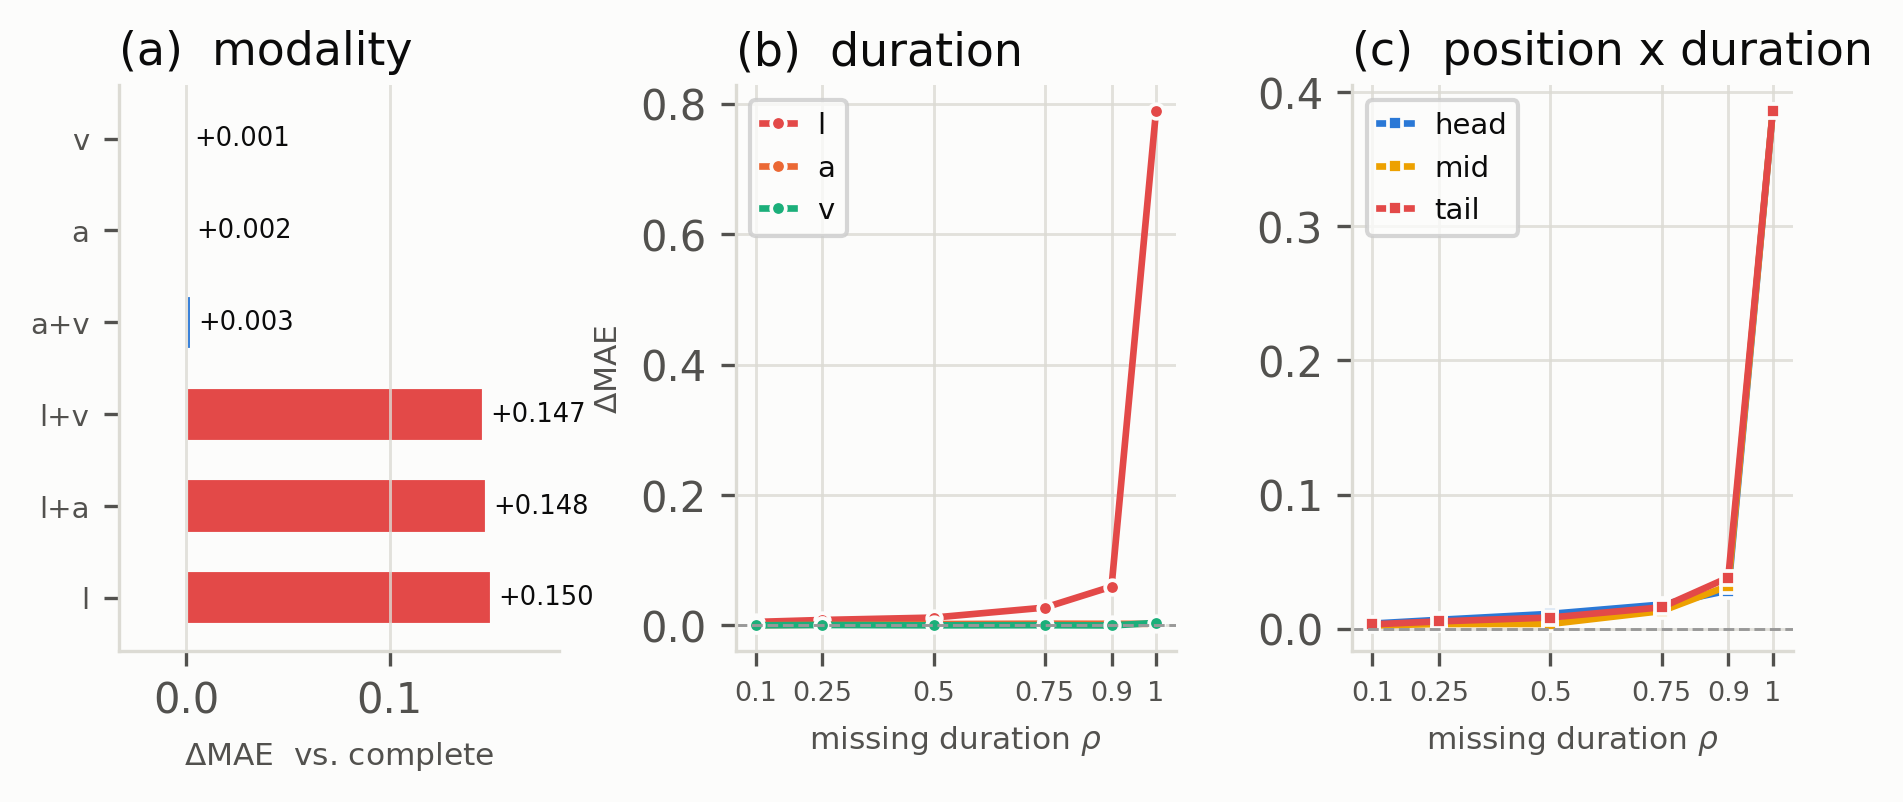
\includegraphics[width=\textwidth]{figures/fig_factor_scan.png}
\caption{三因子扫描结果：(a) 各模态组合的平均 $\Delta\mathrm{MAE}$；(b) 各模态 $\Delta\mathrm{MAE}$ 随时长的变化；(c) 不同位置下 $\Delta\mathrm{MAE}$ 随时长的变化}
\label{fig:factor}
\end{figure}

拆到各模态看，规律完全不同。语言呈现“全有或全无”的形态：缺失90\%以内几乎无感（$\rho=0.9$ 时 $\Delta\mathrm{MAE}$ 仅0.060），一旦接近全缺就断崖式崩溃（$\rho=1.0$ 时为0.789，是前者的13倍）。语音、视觉则全程平缓，始终低于0.006。

我们对语言这种形态的理解是：文本特征是 BERT 的上下文表示，每一帧都编码了整句的信息，即使在补齐位置上也不为零（表\ref{tab:zero}中文本零帧比例为0）。所以只要还剩一部分文本帧，模型就能从中读出整句的情感；也正因为冗余度高，剩余信息一旦不足，就再没有冗余可退，崩溃是断崖式的。语音、视觉的有效帧少（中位21帧）、冗余度低，信息随缺失线性流失，贡献也小，所以曲线平缓。

\subsubsection{位置的影响}

表\ref{tab:pos}按缺失位置分组（每组36个单元）给出了平均 MAE。

\begin{table}[htbp]
\centering
\caption{不同缺失位置下的平均 MAE}
\label{tab:pos}
\begin{tabular}{lccc}
\toprule
位置 & 前部 head & 中部 mid & 尾部 tail \\
\midrule
MAE & 0.7319 & 0.7296 & 0.7324 \\
\bottomrule
\end{tabular}
\end{table}

三者相差不到0.003，远小于时长效应（0.386）。我们原本猜测“句子中部的缺失最要命”，这个假设被数据否定了。这可能与数据的词级对齐有关：序列不是按时间等距采样的，每一帧就是一个词，而情感线索在句中的分布并没有明显的位置偏好；再加上文本帧都是上下文表示，缺了哪一段，其余帧里多少都还留着这段的信息。

\subsubsection{规律小结}

三因子扫描的结论可以归纳为三句话：时长是主因，而不是位置，也不单是“哪个模态”；语言缺失90\%以内几乎无感，接近全缺时 $\Delta\mathrm{MAE}$ 陡增13倍；位置的影响可以忽略。落到应用上，在90\%以内的缺失预算下，应优先保证语言不被整段丢掉，而不必纠结缺失发生在句子的哪个位置。换句话说，“丢了多少”比“丢在哪里”重要得多。

\subsection{附件3的推理结果}\label{sec:att3}

附件3的推理流程与训练时的预处理完全一致：先用 bert-base-uncased 把 text\_bert 重建为文本特征，在标准化之前计算各模态有效长度，再用训练集统计量对语音、视觉做 z-score，最后送入 LDSD-Seg。每条样本输出极性、极性置信度（三分类概率的最大值）、强度和主导模态。30条样本的汇总见表\ref{tab:att3}，逐条结果见附录\ref{app:att3}，分布见图\ref{fig:att3}。

\begin{table}[htbp]
\centering
\caption{附件3推理结果汇总}
\label{tab:att3}
\begin{tabularx}{\textwidth}{lX}
\toprule
项目 & 结果 \\
\midrule
极性分布 & 正向14条，负向11条，中性5条 \\
极性置信度均值 & 0.703 \\
预测强度均值 & $-0.077$ \\
主导模态 & 文本28条；例外为附件3\_14（视觉主导）和附件3\_17（语音主导） \\
\bottomrule
\end{tabularx}
\end{table}

\begin{figure}[htbp]
\centering
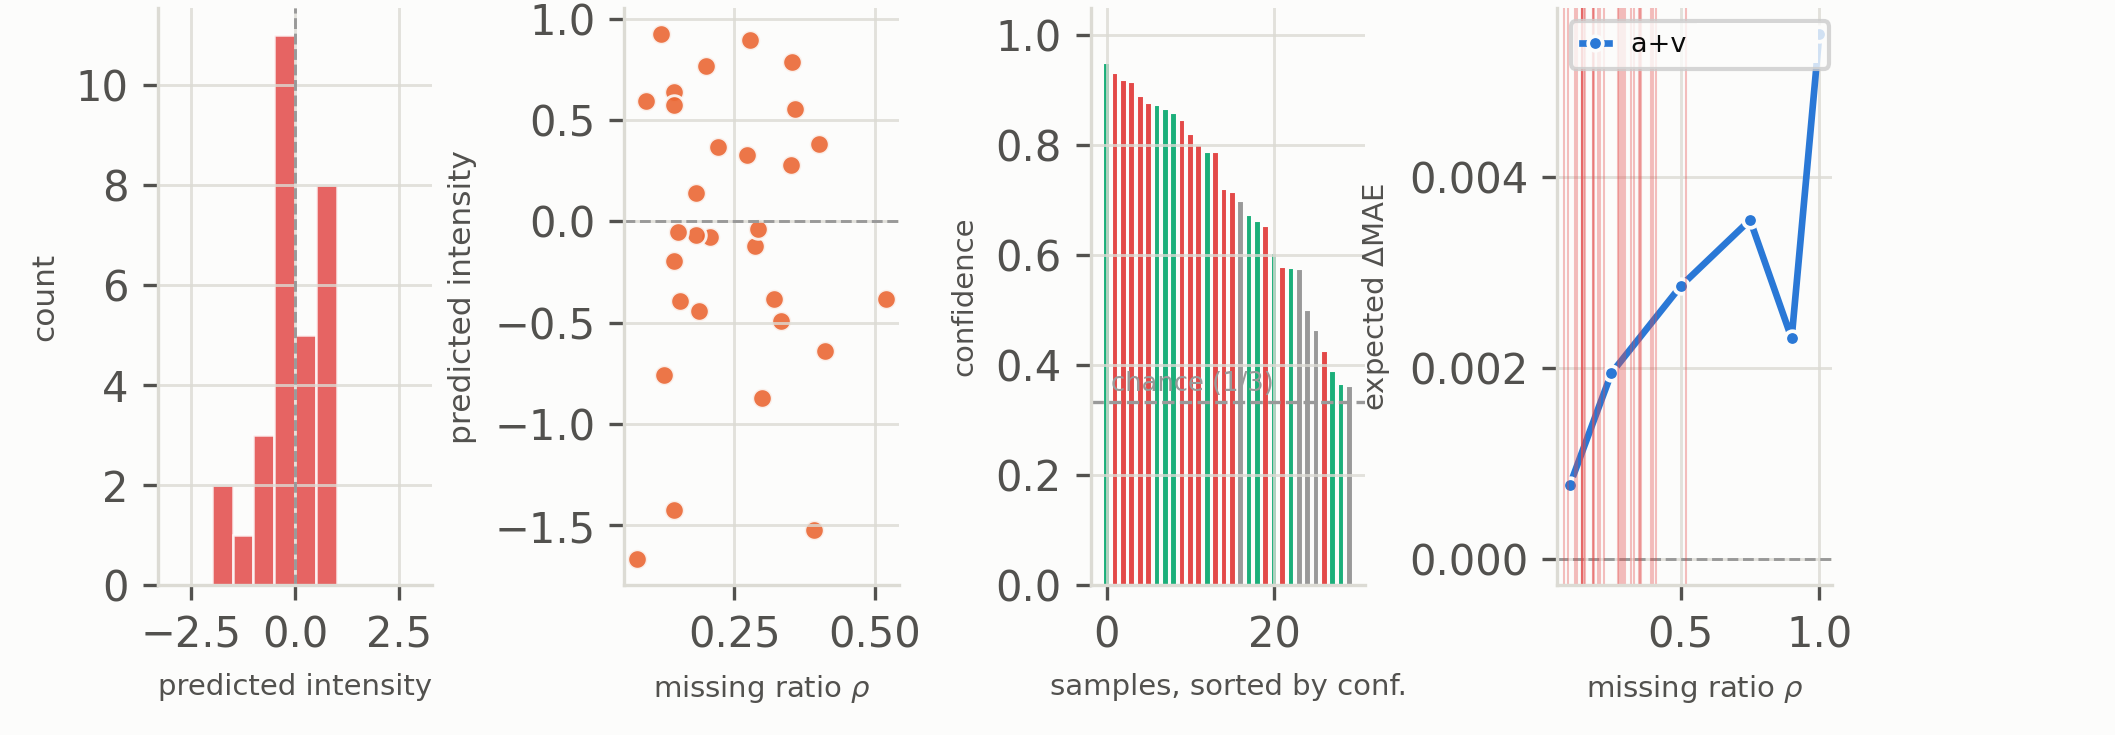
\includegraphics[width=\textwidth]{figures/fig_att3.png}
\caption{附件3推理结果：(a) 预测强度分布；(b) 缺失比例与预测强度；(c) 按置信度排序的极性置信度（红、绿、灰分别为正向、负向、中性）；(d) 各样本缺失比例（竖线）与因子扫描中 $a{+}v$ 缺失的预期 $\Delta\mathrm{MAE}$ 曲线}
\label{fig:att3}
\end{figure}

有几点观察。第一，附件3的缺失全部落在语音和视觉上，缺失比例 $\rho$ 都不超过0.55。对照因子扫描中 $a{+}v$ 缺失的曲线（图\ref{fig:att3}(d)），这个范围内预期的 $\Delta\mathrm{MAE}$ 不超过0.003，远没有到语言的断崖区，所以附件3的缺失对预测的影响应当很小；图\ref{fig:att3}(b)中预测强度与缺失比例之间也看不出明显的趋势。第二，5条中性预测里有4条排在置信度最低的7条之内，中性样本最不“确定”，这与第\ref{sec:robust}节 F1 掉得比准确率快的现象是吻合的。第三，附件3\_14 和附件3\_17 两条的主导模态不是文本，这在30条里比较特殊，建议人工回看。

需要强调的是，附件3没有标签，上面这些只能说明模型输出是否“合理”，不能说明它是否“正确”。附件3预测结果的可信度，主要取决于模型在附件2上的表现。

\subsection{验证集上的错误归因}\label{sec:q2err}

综合前面几节的结果，模型的错误主要来自以下几个方面。

\textbf{（1）类别之间不均衡，缺失越重越明显。}各种条件下 F1-macro 都明显低于 Acc-3；缺失率升高时 F1 掉得更快，$r=0.9$ 时低于随机水平而 Acc-3 仍有50.76\%，说明预测向少数类别集中。附件3中中性预测的置信度普遍偏低，也指向同一个问题：中性与弱正、弱负之间的边界是模型最拿不准的地方。

\textbf{（2）语言接近全缺时误差陡增。}三因子扫描显示，误差几乎全部集中在语言缺失比例接近1的情形，$\rho$ 从0.9到1.0，$\Delta\mathrm{MAE}$ 由0.060跳到0.789。对于只丢语音、视觉的样本，模型几乎不受影响。

\textbf{（3）训练后期过拟合。}图\ref{fig:curve}中验证集 MAE 在第10轮左右最低，之后整体上升，Acc-3 同步下降。3395条训练样本对这样规模的网络来说偏少，固定训练200轮并不是最优的选择。

\textbf{（4）整模态缺失下重建模块的补偿偏“平均”。}组件消融中去掉重建、去掉 AHL 反而略好，说明在一整路信号都缺失时，重建出的内容更接近均值，稀释了判别信息。这也是我们改用连续段训练、并让重建结果进入推理路径的原因。

\subsection{小结}

问题二的核心发现是：题目要求的局部连续缺失在训练数据中基本不存在，照搬文献的缺失设定训练出的鲁棒性并不可靠。围绕这一点，我们从5个候选中筛出了连续段缺失增强（M1）与超模态补洞（M4）两个模块，在同一套分层连续段掩码下把段缺失 F1 从47.26\%提升到61.70\%，验证集上完整模态与段缺失之间的落差从15.6个点缩小到0.1个点。三因子扫描进一步说明，缺失时长是影响性能的主因，语言缺失呈“全有或全无”的形态，位置的影响可以忽略。

% ==================================================================
\section{问题三：可解释性情感预测}\label{sec:q3}
% ==================================================================

问题三不再训练新的网络。解释层直接挂在第\ref{sec:base}章的预测网络外面，网络结构和参数都不改动，这样才能保证“解释的”就是“预测用的”那个模型。

\subsection{把“可解释”落实成可检验的输出}

题目对可解释性的要求是：说明本次判断主要依据了哪些输入，包括模态间的作用差异、主要参考模态，以及各模态中与判断密切相关的局部片段，并且证据能对应到原始材料。我们把它拆成四层，见表\ref{tab:layers}。

\begin{table}[htbp]
\centering
\caption{解释框架的四个层次}
\label{tab:layers}
\begin{tabular}{clll}
\toprule
层次 & 内容 & 主口径 & 输出 \\
\midrule
L0 & 回指 & 帧 $\leftrightarrow$ 词元，式(\ref{eq:align}) & 帧号对应的原文词 \\
L1 & 模态作用程度 & 干预式归因 & $s_l,s_a,s_v$，主导模态，裕度 $\mu$ \\
L2 & 片段级定位 & 滑动窗口遮蔽扫描 & 各模态逐帧重要性 $\mathrm{Imp}_m(t)$ \\
L3 & 证据呈现 & 回指 + 相对位置 & 文本词组；语音、视觉的词级锚点 \\
\bottomrule
\end{tabular}
\end{table}

这里有一个关键的取舍：结论一律由扰动实验给出，注意力权重只用来生成候选和做交叉检验。理由在第\ref{sec:noattn}节展开。

\subsection{L0：帧与词元的回指}

第\ref{sec:align}节已经证明50个序列位置是词级对齐的：第 $t$ 帧对应 $\texttt{input\_ids}$ 的第 $t$ 个词元。因此任何一帧都可以经 \texttt{tokenizer.decode} 还原成原文的词，不需要任何估计。

回指时有一条必须遵守的约束：证据只能从有效帧里选。文本限于实词区间 $[1,L)$，排除 \texttt{[CLS]}、\texttt{[SEP]} 和 \texttt{[PAD]}；语音、视觉限于帧号小于 $L_m$ 的帧。否则填充帧会被当成“关键证据”。这个坑我们实际踩过：第一版解释卡里出现过“\texttt{[PAD] [PAD] [PAD]}”这样的“证据”。原因前面也提到过，文本特征是上下文表示，补齐位置上的向量并不为零，遮蔽它们同样会让输出变化。

对语音和视觉，由于缺少逐词时间戳，我们给出“第 $t$ 个词元处”的词级锚点，同时给出相对位置 $t/L_m$，方便回到原始视频中按说话进度大致定位。

\subsection{L1：干预式模态归因}

对样本 $\mathbf{x}$，把模态 $m$ 按训练时的缺失注入方式整条遮蔽，记为 $\mathbf{x}_{\setminus m}$，比较遮蔽前后的输出：
\begin{align}
\Delta_m^{reg}&=\big|\hat y_{reg}(\mathbf{x})-\hat y_{reg}(\mathbf{x}_{\setminus m})\big|,\label{eq:dreg}\\
\Delta_m^{cls}&=\mathrm{KL}\Big(p(c\,|\,\mathbf{x})\ \big\|\ p(c\,|\,\mathbf{x}_{\setminus m})\Big),\label{eq:dcls}
\end{align}
前者衡量强度预测的偏移，后者衡量极性分布的变化。模态作用程度取分类口径归一化：
\begin{equation}\label{eq:share}
s_m=\frac{\Delta_m^{cls}}{\sum_{m'}\Delta_{m'}^{cls}},\qquad \sum_m s_m=1,\qquad
m^{*}=\arg\max_m s_m,\qquad \mu=s_{(1)}-s_{(2)},
\end{equation}
其中 $m^*$ 为主要参考模态，$s_{(1)}$、$s_{(2)}$ 为从大到小排列的前两个作用程度，$\mu$ 称为判定裕度。回归口径 $\Delta_m^{reg}$ 同时输出，作为辅助参考。

之所以额外报告裕度 $\mu$，是因为“主导模态是文本”这句话本身信息量有限：$s_l=0.95$ 和 $s_l=0.40$ 都会得出同一个结论，但含义差别很大。$\mu$ 小说明两个模态的作用接近，这时读者就不应把“主导模态”看得太重。

这里用遮蔽而不用梯度类方法（如积分梯度\cite{sundararajan2017ig}），还有一个本题特有的原因。积分梯度需要一个“基线输入”，而缺失场景下什么样的输入算“没有信息”本身就不好定义；遮蔽后的输入则正是模型训练时见过的缺失形态（假设(4)的说明），输出变化更可信。

\subsection{L2：片段重要性扫描}

用宽度为 $w$ 的窗口在模态 $m$ 的有效帧上滑动，只遮蔽窗口 $[t,t+w)$ 内的帧，记为 $\mathbf{x}^{[t,t+w)}_{\setminus m}$，定义第 $t$ 帧的片段重要性为
\begin{equation}\label{eq:imp}
\mathrm{Imp}_m(t)=\Big|\hat y_{reg}(\mathbf{x})-\hat y_{reg}\big(\mathbf{x}^{[t,t+w)}_{\setminus m}\big)\Big|
+\Big|p_{(1)}(\mathbf{x})-p_{(1)}\big(\mathbf{x}^{[t,t+w)}_{\setminus m}\big)\Big|,
\end{equation}
其中 $p_{(1)}$ 为遮蔽前预测类别的概率。第一项反映强度的变化，第二项反映对原判断的动摇程度。对主导模态取 $\mathrm{Imp}_m(t)$ 最大的若干帧作为关键证据帧，再经 L0 回指到原文词组或词级锚点。解释层的参数见表\ref{tab:xaiparam}。

\begin{table}[htbp]
\centering
\caption{解释层的主要参数}
\label{tab:xaiparam}
\begin{tabular}{>{\raggedright\arraybackslash}p{4.2cm}>{\raggedright\arraybackslash}p{8.6cm}}
\toprule
参数 & 设置 \\
\midrule
模态遮蔽方式 & 与训练时的缺失注入一致：语音、视觉置零，语言替换为 \texttt{[UNK]} 向量 \\
候选帧范围 & 文本 $[1,L)$；语音、视觉 $t<L_m$ \\
窗口宽度 $w$、证据帧数 $k$、稳定性检验噪声强度 & \todo{从配置文件抄录} \\
\bottomrule
\end{tabular}
\end{table}

\subsection{为什么不用注意力，以及融合层的等价重写}\label{sec:noattn}

式(\ref{eq:alpha})(\ref{eq:beta})中的 $\alpha$、$\beta$ 看上去就是现成的“解释”：它告诉我们语言的每个词关注了语音、视觉的哪些帧。但文献\cite{jain2019attention}的实验表明，注意力权重与预测的因果贡献并不必然一致，换一组差别很大的注意力分布，预测可以几乎不变。所以本文的结论全部来自扰动实验，注意力只做两件事：为片段扫描提供候选，以及与扰动结果做交叉检验。

即便只用来交叉检验，也得先把注意力取出来，这里遇到了一个工程问题。融合层使用的是 PyTorch 的 \texttt{TransformerDecoderLayer}，它内部调用注意力时设置了 \texttt{need\_weights=False}，即使挂上前向钩子，拿到的也只是 \texttt{None}。我们用显式的解码层重写了 \texttt{CrossModalFusion}，子模块命名与官方实现完全一致，因此可以直接加载原来训练好的参数。为了证明重写后的层与原层等价，做了三项检查，见表\ref{tab:equiv}。

\begin{table}[htbp]
\centering
\caption{重写融合层的等价性检查}
\label{tab:equiv}
\begin{tabular}{ll}
\toprule
检查项 & 结果 \\
\midrule
与原层的输出差异 & 最大绝对差 $4.77\times10^{-7}$（float32 舍入量级） \\
\texttt{state\_dict} 键名 & 完全不变，原检查点可直接加载 \\
开启注意力输出对预测的影响 & 逐元素相等，$\max|\Delta\hat y_{reg}|=0$ \\
\bottomrule
\end{tabular}
\end{table}

做这三项检查的原因很简单：可解释性分析报告的必须是真正在用的那个模型，而不是一个行为略有不同的近似副本，否则“解释”和“预测”就对不上了。

\subsection{解释质量的量化检验}

解释本身也需要被检验。我们用三个指标衡量解释的质量，结果见表\ref{tab:xaiquality}。
\begin{itemize}
\item \textbf{忠实性比值}：遮蔽重要性最高的 $k$ 个证据帧所引起的预测变化，除以遮蔽 $k$ 个随机有效帧所引起的预测变化。比值越大，说明挑出来的证据确实比随便挑的帧更重要。
\item \textbf{稳定性}：对输入加入微小噪声后重新计算重要性曲线，与原曲线的 Spearman 秩相关系数。越接近1，说明解释不会因为微小扰动而大幅改变。
\item \textbf{充分性偏移}：只保留重要性最高的3帧、遮蔽其余帧时，预测相对原预测的偏移量。越小说明少数证据帧就足以支撑原判断。
\end{itemize}

\begin{table}[htbp]
\centering
\caption{解释质量指标}
\label{tab:xaiquality}
\begin{tabularx}{\textwidth}{lcX}
\toprule
指标 & 数值 & 含义 \\
\midrule
忠实性比值 & 2.88 & 遮蔽 top-$k$ 证据造成的预测变化是随机帧的2.88倍 \\
稳定性（Spearman） & 0.9973 & 输入加噪后重要性曲线几乎不变 \\
充分性偏移 & 0.7068 & 只保留 top-3 帧时预测的偏移量 \\
\bottomrule
\end{tabularx}
\end{table}

前两项的结果比较理想：挑出的证据明显比随机帧重要，而且解释很稳定。第三项则提醒我们，只留3帧时预测偏移了0.7068，说明少数几帧并不足以单独支撑判断，模型依赖的信息是分散在整句中的。这与第\ref{sec:factor}节看到的语言高冗余是一致的。所以对文本证据更准确的读法是“模型最依赖的区域”，而不是“决定情感的那几个词”。

\subsection{三模态作用差异}

在验证集的192条样本上统计模态作用程度，结果见表\ref{tab:modshare}。

\begin{table}[htbp]
\centering
\caption{验证集（$n=192$）上的三模态作用程度}
\label{tab:modshare}
\begin{tabular}{lccc}
\toprule
 & 文本 & 语音 & 视觉 \\
\midrule
平均作用程度 $\bar s_m$ & \textbf{0.871} & 0.049 & 0.080 \\
作为主导模态的样本占比 & \textbf{92\%} & 4\% & 5\% \\
\bottomrule
\end{tabular}
\end{table}

注：占比经四舍五入，合计略超100\%。

这是我们最看重的一次交叉验证。干预式归因是在单个样本上做的，第\ref{sec:ablation}节的模态消融是在整个数据集上重新评测的，两条技术路线完全不同，却给出了同一个答案：语言是主导。这说明归因的口径是可信的。

表中还有一个值得注意的细节：视觉的平均作用程度（0.080）高于语音（0.049），可模态消融里去掉语音的损失（F1 $-3.1$）反而比去掉视觉（$+2.5$）大。两者并不矛盾。作用程度衡量的是“遮掉之后输出变了多少”，并不区分变得更准还是更差；视觉让输出变动较多，但这种变动未必朝着正确的方向，去掉视觉后 F1 略升也说明它带来的一部分是噪声。

\subsection{典型样本的解释}\label{sec:card}

图\ref{fig:interp}展示了测试集中的几条样本。左图是第0号样本三个模态的片段重要性曲线，横轴是帧号（即词元序号），竖线标出了各模态的关键证据帧；中图是第0～5号样本的模态作用程度；右图是这6条样本各模态的 $\Delta^{cls}$。

\begin{figure}[htbp]
\centering
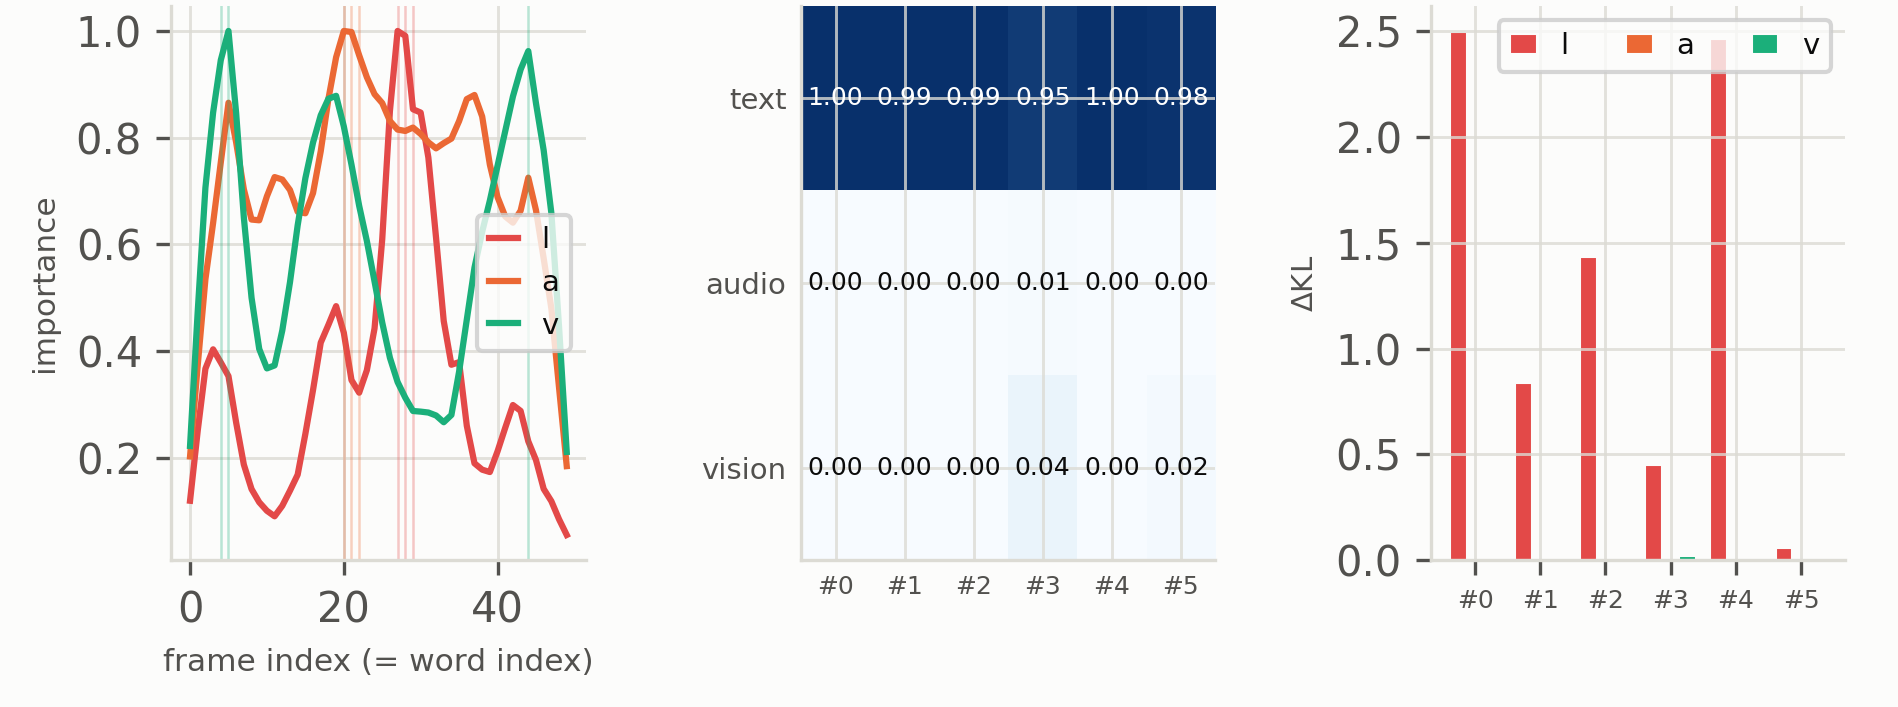
\includegraphics[width=\textwidth]{figures/fig_interpret.png}
\caption{测试样本的解释结果。左：第0号样本的片段重要性（l、a、v 分别为文本、语音、视觉）；中：第0～5号样本的模态作用程度 $s_m$；右：各模态遮蔽后的 $\Delta^{cls}$}
\label{fig:interp}
\end{figure}

从中图看，6条样本的文本作用程度都在0.95以上；语音、视觉只在第3号（视觉0.04、语音0.01）和第5号（视觉0.02）样本上有一点份额。右图说明文本主导的强弱在样本之间差别很大：第0号和第4号遮掉文本后 $\Delta^{cls}$ 接近2.5，第5号只有0.05左右，尽管后者的文本作用程度也有0.98。这正是需要同时看作用程度和绝对效应量的原因：作用程度是相对值，只说明“谁更重要”，而 $\Delta^{cls}$ 说明“整体有多重要”。

左图中文本的重要性在第27～29帧附近出现尖峰，这几帧就是该样本的文本关键证据，回指后即为对应位置的原文词组。

题目要求的解释卡包含预测结果、三模态作用程度、主要参考模态和关键证据定位。以附件4中可在附件2找回真值的第12号样本为例，解释卡如表\ref{tab:card}所示。

\begin{table}[htbp]
\centering
\caption{解释卡示例：附件4第12号样本}
\label{tab:card}
\begin{tabular}{>{\raggedright\arraybackslash}p{3.2cm}>{\raggedright\arraybackslash}p{9.6cm}}
\toprule
字段 & 内容 \\
\midrule
预测极性 & Negative（负向）；附件2中的真值同为 Negative \\
预测强度 & $-1.114$；真值 $-0.667$ \\
主要参考模态 & 文本；判定裕度 $\mu=$ \todo{见 json} \\
三模态作用程度 & $s_l=$ \todo{见 json}，$s_a=$ \todo{见 json}，$s_v=$ \todo{见 json} \\
文本关键证据 & “an individual previously”（词元位置 \todo{见 json}） \\
语音、视觉锚点 & 与文本证据同位置的帧，相对位置 $t/L_m=$ \todo{见 json} \\
复核方法 & 按帧号取 \texttt{input\_ids}，用 \texttt{tokenizer.decode} 还原原文；在原始视频中找到说出该词组的时刻，回看对应的语音与表情 \\
\bottomrule
\end{tabular}
\end{table}

\subsection{附件4的预测与解释结果}\label{sec:att4}

附件4的20条样本三模态完整，按与附件2相同的预处理送入网络，每条输出极性、强度、三模态作用程度、主导模态及裕度、关键证据帧和回指词组。结果分布见图\ref{fig:att4}，逐条结果见附录\ref{app:att4}，完整解释卡存于 attachment4\_explanations.json。

\begin{figure}[htbp]
\centering
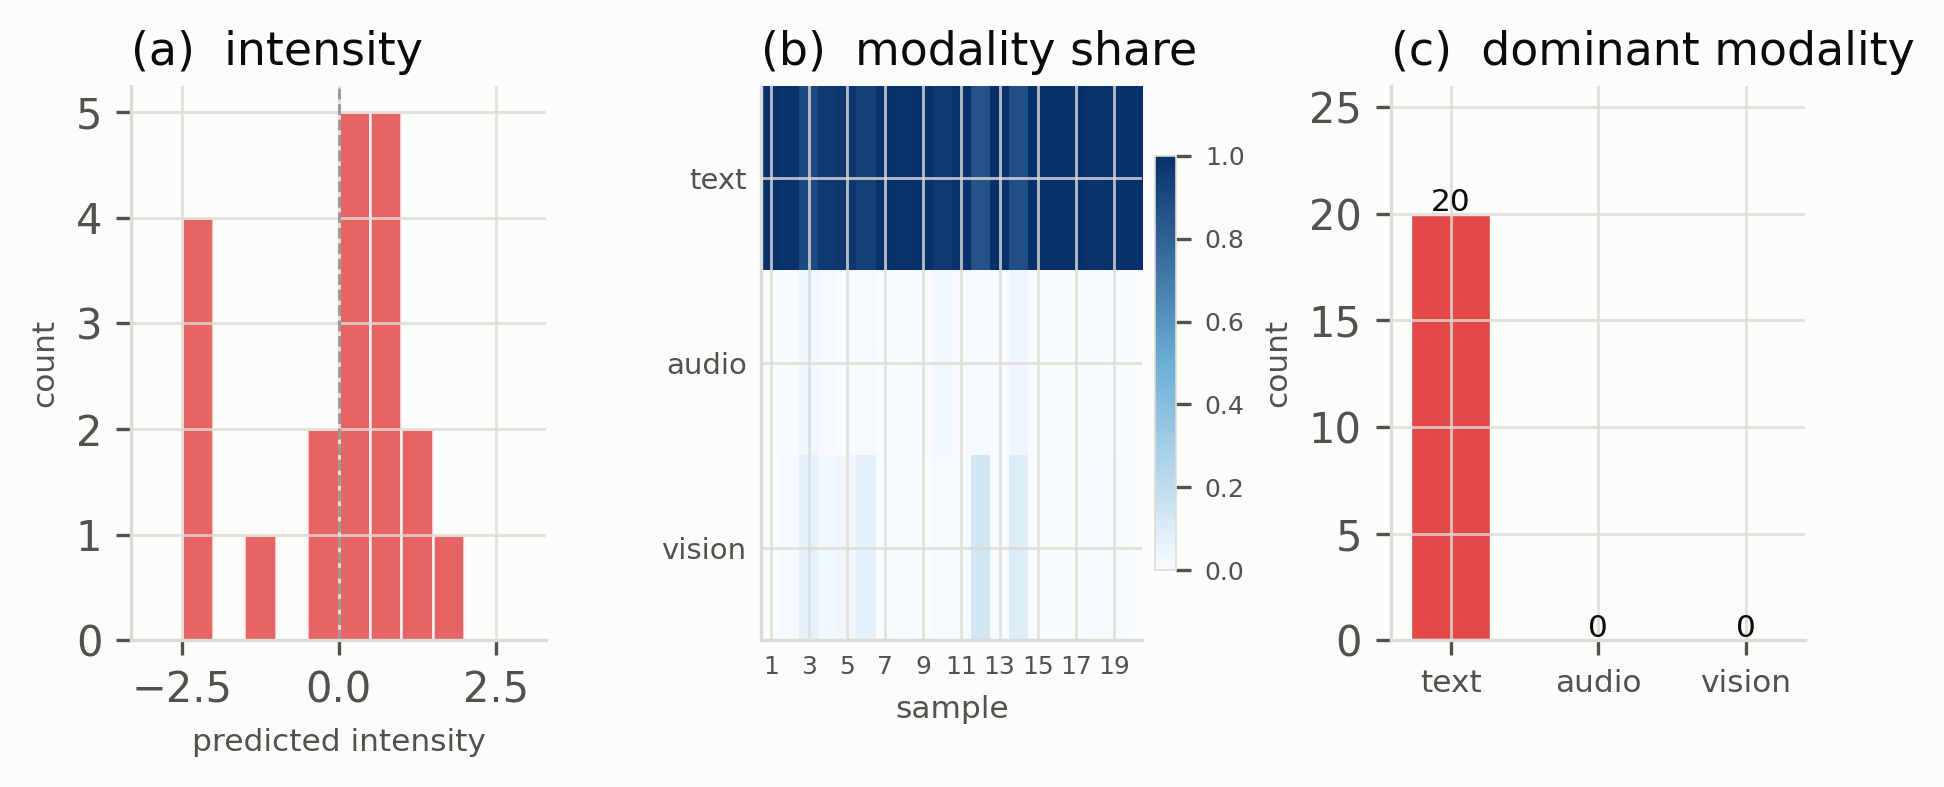
\includegraphics[width=\textwidth]{figures/fig_att4.png}
\caption{附件4推理结果：(a) 预测强度分布；(b) 各样本的模态作用程度；(c) 主导模态统计}
\label{fig:att4}
\end{figure}

20条样本的主导模态全部是文本，判定裕度均大于0.15，也就是说模型对每条样本都有明确的模态偏好。视觉在个别样本上占到了一定比例（图\ref{fig:att4}(b)中的浅色格），但都没有达到主导。预测强度的分布偏向两端，有4条落在$-2$以下的强负向区间。

附件4没有标签，但其中5条可以按编号在附件2里精确找回真值，可以当作一个很小的检验集，结果见表\ref{tab:att4match}。

\begin{table}[htbp]
\centering
\caption{附件4中可找回真值的5条样本}
\label{tab:att4match}
\begin{tabular}{cccccl}
\toprule
样本 & 预测极性 & 真值极性 & 预测强度 & 真值强度 & 文本关键证据 \\
\midrule
03 & Negative & Negative & $-0.402$ & $-0.333$ & “justwest don” \\
07 & Positive & Positive & $+0.946$ & $+0.667$ & “topics growing hobby” \\
08 & Positive & Positive & $+0.827$ & $+0.333$ & “to tonight ,” \\
12 & Negative & Negative & $-1.114$ & $-0.667$ & “an individual previously” \\
15 & Positive & Positive & $+1.379$ & $+1.000$ & “their , transform” \\
\bottomrule
\end{tabular}
\end{table}

5条样本的极性全部判对，强度 MAE 为0.3334。

\subsection{错误归因}\label{sec:q3err}

\textbf{（1）强度被系统性放大。}表\ref{tab:att4match}中5条样本的预测强度，绝对值全部大于真值，平均高出约0.33，强度 MAE 几乎全部来自这种同方向的偏差，例如08号预测$+0.827$，真值只有$+0.333$。样本只有5条，还不能下定论，但方向一致这一点值得重视。一种可能的解释是：真值是多名标注者的平均，标注者意见不一时平均值会被拉向0，而模型学到的是“这类说法通常有多强”。如果这个偏差在验证集上也成立，可以在验证集上拟合一个斜率小于1的线性校准来修正。

\textbf{（2）文本证据不一定是“情感词”。}表\ref{tab:att4match}的证据里有标点和虚词（“to tonight ,”、“their , transform”），也有不完整的词形（“justwest don”，BERT 按子词切分，回指出来的可能是半个词）。这和上文充分性偏移的结论一致：文本帧是上下文表示，遮掉一个窗口去掉的不只是这几个词本身，还有它们承载的上下文信息。因此文本证据应当理解为“模型最依赖的位置”，阅读时最好结合前后文。

\textbf{（3）语音、视觉的证据只能到词级。}数据中没有逐词时间戳，我们给出的是词级锚点和相对位置，不是绝对秒数。这是数据本身的限制，我们没有用“平均词长乘总时长”去凑一个秒数，因为那样得到的数字无法复核。

\textbf{（4）解释暴露了模型对文本的高度依赖。}92\%的样本以文本为主导，这是模型的真实行为，解释如实反映了它。反过来说，如果某条样本的转写文本有错，模型很可能跟着出错，而这类样本的解释卡会显示“文本主导”，读者据此就能意识到应当先核对转写。这也是可解释性在实际使用中的价值所在。

\subsection{小结}

问题三在不改动网络的前提下，用“干预 + 回指”的方式给出了可量化、可复核的解释：模态作用程度由遮蔽后的输出变化归一化得到，关键证据由滑动窗口扫描定位，再借助帧—词元对应还原到原文。忠实性比值2.88、稳定性0.9973说明解释是可靠的；单样本归因与整体消融两条独立路线得到同一个结论，互相印证了口径的可信度。主要的不足在于语音、视觉只能定位到词级，以及模型存在放大情感强度的倾向。

% ==================================================================
\section{模型评价}\label{sec:eval}
% ==================================================================

\subsection{模型的优点}

\begin{enumerate}[label=\arabic*.]
\item \textbf{三种对齐共用一个算子、一个接口。}问题一的三种方案只在“时间轴怎么定义”上不同，输出形状完全一致，下游可以直接切换；其中口径H复刻了附件2的词级对齐，每个位置都能回指到原文的词。
\item \textbf{有效时段的判据更贴合情感表达。}说话者人脸跟踪方案以“说话者的脸是否可见”划定有效时段，既剔除了无人时段，又保留了不说话时的表情；按声音判定只剩32\%的时长，而该判据平均保留93\%，语音、视觉非零位置分别为48.0和47.5。
\item \textbf{先查数据，再定方法。}建模前逐帧核查了附件2—附件4，发现训练数据与专项测试集的缺失形态根本不同，并据此改写了缺失模拟方式。仅这一项（M1）不改网络结构，就让段缺失 F1 提升了9.4个点。同一轮核查还确认了帧与词元的一一对应，为问题三的精确回指打下了基础。
\item \textbf{模块去留由数据决定。}我们为局部连续缺失准备了5个候选模块，按统一掩码逐级叠加筛选，最终只保留2个。被淘汰模块的结果和筛选过程中走过的弯路（在坏配置上叠加导致一轮结果作废）都完整保留在正文中。
\item \textbf{改进落在最难的情形上。}LDSD-Seg 在长段缺失上的 MAE 降幅（0.066）大于整体（0.047），验证集上完整模态与段缺失之间的 F1 落差由15.6个点缩小到0.1个点，鲁棒性的提升不是靠容易样本刷出来的。
\item \textbf{规律分析有自检。}三因子扫描前设置了“语言全缺必须最差”的校验项，靠它发现并修正了两处会导致错误结论的设计问题，避免了把 bug 当成发现写进报告。
\item \textbf{解释对得上、查得到。}解释层不改网络，融合层重写后与原层的最大输出差为 $4.77\times10^{-7}$；文本证据精确回指到词元，可当场人工核对；忠实性、稳定性两项指标表现良好，单样本归因与整体消融两条路线的结论一致。
\end{enumerate}

\subsection{模型的缺点}

\begin{enumerate}[label=\arabic*.]
\item \textbf{问题一的对齐依赖“词匀速发音”近似。}方法一、二在没有逐词时间戳的情况下按均匀发音给词元分配时刻，语速变化大时会有词级误差；方法三的说话者身份靠人脸面积匹配，面积比阈值0.4是经验值，没有逐样本自适应。
\item \textbf{对齐质量没有在下游任务上检验。}问题一的语音、视觉特征与附件2不在同一个特征空间，附件1又只有100条，我们只用非零位置数等结构指标评价了三种方案，没有比较它们对情感预测的实际影响；视觉特征也只用了人脸几何与像素统计量，对细微表情的刻画偏粗。
\item \textbf{语音、视觉证据只能定位到词级。}数据没有逐词时间戳，本文没有利用附件4的原始视频做语音—文本强制对齐，因此给不出秒级的语音时段和视觉关键帧。
\item \textbf{“重建有益”只得到部分复现。}在整模态缺失下，去掉重建或去掉 AHL 后 MAE 反而略好。本文给出了可能的解释，但由于时间有限，没有设计专门的实验去验证。
\item \textbf{结果多为单次运行。}同一个 M1+M4 配置在筛选实验与确认实验中的段缺失 F1 相差约1.5个点，说明存在运行间波动，而本文没有做多随机种子重复、也没有给出置信区间。
\item \textbf{训练轮数没有调优。}验证曲线显示模型在训练中后期出现过拟合，固定训练200轮并非最优，本文没有系统比较早停的效果。
\item \textbf{专项测试集缺少标签。}附件3、4的可信度只能借助附件2上的表现间接判断；强度被放大的现象只在附件4的5条可找回样本上观察到，样本太少。
\end{enumerate}

\subsection{改进方向}

针对上面的不足，后续可以从几个方面改进。第一，引入语音识别与强制对齐工具，得到逐词时间戳。这一步能同时改进两处：问题一的方法一、二不再依赖“词匀速发音”的近似；问题三的词级锚点可以换算成秒级的语音时段和视频关键帧，证据定位直接落到原始素材上。视觉方面，可以在人脸框内再接一个面部动作单元或表情特征提取器，补足对细微表情的刻画。第二，按验证集指标早停，并用多个随机种子重复主要实验，报告均值和区间，让小幅差异的比较更有依据。第三，在验证集上检查强度放大是否普遍存在，若存在则拟合线性校准。第四，模型对文本的依赖过重，一旦转写出错就容易被带偏，可以在训练时提高文本连续段缺失的比例，迫使模型更多地利用语音和视觉；中段缺失改善最小的原因也值得进一步分析。


\bibliographystyle{gmcm}
\bibliography{refs}

\newpage
\appendix
\makeatletter
\renewcommand\secdot{}
\renewcommand\thesubsection{\Alph{section}.\arabic{subsection}}
\makeatother
\addtocontents{toc}{\protect\renewcommand\protect\tocsecdot{}}
% ==================================================================
\section{支撑材料与运行环境}\label{app:env}
% ==================================================================

\subsection{支撑材料清单}

表\ref{tab:files}列出了随论文提交的支撑材料。

\begin{table}[htbp]
\centering
\caption{支撑材料清单}
\label{tab:files}
\begin{tabularx}{\textwidth}{l>{\raggedright\arraybackslash}X}
\toprule
类别 & 文件 \\
\midrule
问题一代码包 & q1\_code\_package/：step1\_extract（方法一）、step1\_time50（方法二）、step1\_vad50（方法三）、eval（评估与可视化），含 README 与 requirements.txt \\
问题一模型权重 & models/bert-base-uncased、models/yunet/face\_detection\_yunet\_2023mar.onnx \\
问题一特征文件 & 三种方案各100个 .npz，目录见第\ref{sec:q1file}节 \\
附件1汇总脚本 & tools/make\_q1\_table.py（由 .npz 生成附录\ref{app:q1}的全量汇总表） \\
建模 Notebook & ldsd\_notebook.ipynb（69个单元格，15节），可在 Kaggle 上一键运行 \\
数据核查 Notebook & audit\_notebook.ipynb \\
模型参数 & ldsd\_main.pt（9.08 MB）\newline ldsd\_segment.pt（10.16 MB）\newline ablation\_models.pt（78.49 MB，9个消融模型打包） \\
预测与解释 & attachment3\_predictions.csv，attachment3\_explanations.json\newline attachment4\_predictions.csv，attachment4\_explanations.json \\
实验脚本 & exp\_segment.py（候选模块筛选），exp\_factors.py（三因子扫描） \\
绘图脚本 & make\_architecture\_fig.py，make\_charts.py \\
结果表 & summary\_all.csv，robustness.csv，factor\_scan\_agg.csv 等共12份 \\
\bottomrule
\end{tabularx}
\end{table}

\subsection{运行环境与运行说明}

\textbf{问题一。}在本地 Windows 环境运行，只需 CPU。
\begin{itemize}
\item 环境：Python 3.10（conda 环境），PyTorch 使用 CPU 版，其余依赖按 requirements.txt 安装；librosa、OpenCV、transformers、ffmpeg 的版本号为 \todo{按 requirements.txt 填写}。
\item 必设环境变量：\texttt{KMP\_DUPLICATE\_LIB\_OK=TRUE}（避免 OpenMP 重复加载导致崩溃）、\texttt{PYTHONIOENCODING=utf-8}（中文输出不乱码）；数据不在默认位置时另设 \texttt{DATA\_ROOT}。
\item 运行方式：分别进入 step1\_extract、step1\_time50、step1\_vad50 目录执行 \texttt{python main.py}（加 \texttt{--limit 3} 可先调试前3条），三种方案跑完后在 eval 目录执行 eval\_align.py 得到表\ref{tab:q1eval}，执行 visualize\_sample.py 得到典型样本图；最后运行 tools/make\_q1\_table.py 生成附录\ref{app:q1}的汇总表。
\item 随机种子：SEED = 2026。
\end{itemize}

\textbf{问题二、三。}全部实验在 Kaggle 提供的 GPU 环境上完成，全量运行总耗时 7772.6 s（约2.16 h）。
\begin{itemize}
\item 软件版本：Python、PyTorch、transformers 的版本为 \todo{按运行环境填写}；文本编码器为 bert-base-uncased。
\item 运行入口：ldsd\_notebook.ipynb 按顺序执行即可复现全部结果；数据上传、BERT 依赖、运行方式和各步耗时见 README.md 中的“Kaggle 全量运行指南”。
\item 随机种子：\todo{填写实际使用的随机种子}。固定随机种子是为了保证结果可复现。
\item 数据处理规则：有效长度在标准化之前从原始特征计算（式(\ref{eq:validlen})）；语音、视觉使用训练集统计量标准化（式(\ref{eq:zscore})）；附件3的文本由 text\_bert 经 bert-base-uncased 重建。
\end{itemize}

% ==================================================================
\section{核心算法伪代码}\label{app:algo}
% ==================================================================

\begin{algorithm}[H]
\caption{说话者人脸跟踪与有效时段对齐（问题一方法三）}
\label{alg:m3}
\begin{algorithmic}[1]
\Require 视频片段（时长 $D$），三路帧级特征，$\kappa=0.4$
\Ensure 对齐后的 text、audio、vision（各50个位置）
\State 计算语音短时能量 $e_j$，$e_j\ge0.05\max e$ 判为语音帧；剔除短于0.15 s 的语音段，填补短于0.25 s 的静音间隙
\State 在“语音帧且检测到人脸”的帧中取面积最大的人脸，记典型面积 $A_s$
\For{每个视频帧 $\tau$}
  \State $v(\tau)\gets\mathbb{1}[\text{检测到人脸}\wedge A(\tau)\ge\kappa A_s]$
\EndFor
\If{$v\equiv0$} \State 退化为全程50等分（方法二）并返回 \EndIf
\State 拼接可见时段得 $\varphi(\tau)=\int_0^\tau v$，$D_{eff}=\varphi(D)$，锚点 $a_k=kD_{eff}/49$
\State 三路只保留可见时段内的帧（词元按均匀发音取时刻），时间戳映射为 $\varphi(\tau_i)$
\State 按式(\ref{eq:tri})把三路特征重采样到 $a_0,\dots,a_{49}$
\State \Return text $(50,768)$，audio $(50,74)$，vision $(50,35)$
\end{algorithmic}
\end{algorithm}

\begin{algorithm}[H]
\caption{连续段缺失掩码生成（M1）}
\label{alg:m1}
\begin{algorithmic}[1]
\Require 序列长度 $T$，缺失率 $r$，Dirichlet 浓度 $0.6$
\Ensure 缺失掩码 $M\in\{0,1\}^T$
\State $M\gets\mathbf{0}$；抽取段数 $k\sim\mathcal{U}\{1,2,3\}$
\State 抽取段长比例 $(\rho_1,\dots,\rho_k)\sim\mathrm{Dirichlet}(0.6\cdot\mathbf{1}_k)$
\State 将 $[0,T)$ 划分为 $k$ 个互不相交的区块 $B_1,\dots,B_k$
\For{$j=1$ \textbf{to} $k$}
  \State $\ell_j\gets\max\big(1,\lfloor\rho_j\,rT\rfloor\big)$
  \State 在区块 $B_j$ 内选取起点 $a_j$，使 $[a_j,a_j+\ell_j)$ 落在 $B_j$ 中
  \State $M[a_j:a_j+\ell_j]\gets 1$
\EndFor
\State \Return $M$
\end{algorithmic}
\end{algorithm}

\begin{algorithm}[H]
\caption{干预式模态归因与片段扫描（问题三）}
\label{alg:xai}
\begin{algorithmic}[1]
\Require 样本 $\mathbf{x}$，训练好的网络 $f$，窗口宽度 $w$，证据帧数 $k$
\Ensure 作用程度 $s_m$，主导模态 $m^*$，裕度 $\mu$，关键证据
\State 计算原始输出 $\hat y_{reg}(\mathbf{x})$、$p(c\,|\,\mathbf{x})$
\For{$m\in\{l,a,v\}$}
  \State 按训练时的缺失注入方式整条遮蔽模态 $m$，得到 $\mathbf{x}_{\setminus m}$
  \State 按式(\ref{eq:dreg})(\ref{eq:dcls})计算 $\Delta_m^{reg}$、$\Delta_m^{cls}$
\EndFor
\State 按式(\ref{eq:share})计算 $s_m$、$m^*$、$\mu$
\For{$m\in\{l,a,v\}$}
  \For{有效帧 $t$（文本 $t\in[1,L)$，语音、视觉 $t<L_m$）}
    \State 遮蔽模态 $m$ 的窗口 $[t,t+w)$，按式(\ref{eq:imp})计算 $\mathrm{Imp}_m(t)$
  \EndFor
\EndFor
\State 取主导模态中 $\mathrm{Imp}$ 最大的 $k$ 帧，经帧—词元对应回指为原文词组或词级锚点
\State \Return 解释卡
\end{algorithmic}
\end{algorithm}

% ==================================================================
\section{附件1全量特征提取结果}\label{app:q1}
% ==================================================================

下表由 tools/make\_q1\_table.py 读取三种方案的 .npz 文件后生成（results/q1\_summary.csv）。所有样本的特征维度均为 text $(50,768)$、audio $(50,74)$、vision $(50,35)$；对齐粒度方法一为词级，方法二、三为50个时间桶。表头含义：dur 为片段时长（s），L\_txt 为有效词元数，eff\_s 与 eff\_ratio 为方法三的有效时长与占比，n\_seg 为说话段数，nzA/nzV 为语音/视觉非零位置数，后缀 H、T50、V50 分别对应方法一、二、三。

\IfFileExists{results/q1_summary.csv}{%
  {\scriptsize\setlength{\tabcolsep}{2.5pt}\renewcommand{\arraystretch}{1.05}%
  \csvautolongtable[respect all]{results/q1_summary.csv}}%
}{%
  \todo{运行 tools/make\_q1\_table.py 生成 results/q1\_summary.csv 后重新编译，这里会自动生成100条样本的汇总表}%
}

% ==================================================================
\section{附件3全量预测结果}\label{app:att3}
% ==================================================================

下表由 results/attachment3\_predictions.csv 自动生成。

\IfFileExists{results/attachment3_predictions.csv}{%
  {\scriptsize\setlength{\tabcolsep}{3pt}\renewcommand{\arraystretch}{1.1}%
  \csvautolongtable[respect all]{results/attachment3_predictions.csv}}%
}{%
  \todo{把 attachment3\_predictions.csv 放到 results/ 目录后重新编译，这里会自动生成30条样本的全量结果表}%
}

% ==================================================================
\section{附件4全量预测与解释结果}\label{app:att4}
% ==================================================================

下表由 results/attachment4\_predictions.csv 自动生成，完整解释卡见 attachment4\_explanations.json。

\IfFileExists{results/attachment4_predictions.csv}{%
  {\scriptsize\setlength{\tabcolsep}{3pt}\renewcommand{\arraystretch}{1.1}%
  \csvautolongtable[respect all]{results/attachment4_predictions.csv}}%
}{%
  \todo{把 attachment4\_predictions.csv 放到 results/ 目录后重新编译，这里会自动生成20条样本的全量结果表}%
}


\end{document}
